%Dokumenteinstellungen und Anpassungen
%Dokumentenklasse "scrbook" - Erweitert um den Verweis auf die Verzeichnisse und Texteigenschaften
\documentclass[chapterprefix=false, 12pt, a4paper, oneside, parskip=half, listof=totoc, bibliography=totoc, numbers=noendperiod]{scrbook}

\usepackage{sidecap}
\usepackage{caption}
\usepackage{subcaption}

%Anpassung der Seitenränder (Standard bottom ca. 52mm anbzüglich von ca. 4mm für die nach oben rechts gewanderte Seitenzahl)
\usepackage[bottom=48mm,left=25mm,right=25mm]{geometry}

%Tweaks für scrbook
\usepackage{scrhack}

%Blindtext
\usepackage{blindtext}

%Erlaubt unteranderem Umbrücke captions
\usepackage{caption}

%Stichwortverzeichnis
\usepackage{imakeidx}

%Kompakte Listen
\usepackage{paralist}

%Zitate besser formatieren und darstellen
\usepackage{epigraph}

%Glossar, Stichworverzeichnis (Akronyme werden als eigene Liste aufgeführt)
\usepackage[toc, acronym]{glossaries} 

%Anpassung von Kopf- und Fußzeile
%beinflusst die erste Seite des Kapitels
\usepackage[automark,headsepline]{scrlayer-scrpage}
\automark{chapter}
\ihead{\leftmark}
\chead{}
\ohead{\thepage}
\ifoot*{}
\cfoot[\thepage]{}
\cfoot*{}
\ofoot*{\thepage}
\ofoot{}
\pagestyle{scrheadings}

%Auskommentieren für die Verkleinerung des vertikalen Abstandes eines neuen Kapitels
%\renewcommand*{\chapterheadstartvskip}{\vspace*{.25\baselineskip}}

%Zeilenabstand 1,5
\usepackage[onehalfspacing]{setspace}

%Verbesserte Darstellung der Buchstaben zueinander
\usepackage[stretch=10]{microtype}

%Deutsche Bezeichnungen für angezeigte Namen (z.B. Innhaltsverzeichnis etc.)
\usepackage[english]{babel}

%Unterstützung von Umlauten und anderen Sonderzeichen (UTF-8)
\usepackage{lmodern}
\usepackage[utf8]{luainputenc}
\usepackage[T1]{fontenc}

%Einfachere Zitate
\usepackage{epigraph}

%Unterstützung der H positionierung (keine automatische Verschiebung eingefügter Elemente)
\usepackage{float} 

%Erlaubt Umbrüche innerhalb von Tabellen
\usepackage{tabularx}

%Erlaubt Seitenumbrüche innerhalb von Tabellen
\usepackage{longtable}

%Erlaubt die Darstellung von Sourcecode mit Highlighting
\usepackage{listings}

%Definierung eigener Farben bei nutzung eines selbst vergebene Namens
\usepackage[table,xcdraw]{xcolor}

%Vektorgrafiken
\usepackage{tikz}

%Grafiken (wie jpg, png, etc.)
\usepackage{graphicx}

%Grafiken von Text umlaufen lassen
\usepackage{wrapfig}

%Ermöglicht Verknüpfungen innerhalb des Dokumentes (e.g. for PDF), Links werden durch "hidelink" nicht explizit hervorgehoben
\usepackage[hidelinks]{hyperref}

%Einbindung und Verwaltung von Literaturverzeichnissen
\usepackage{csquotes} %wird von biber benötigt
\usepackage[style=alphabetic, backend=biber, bibencoding=ascii]{biblatex}
\addbibresource{references/references.bib}
%Anpassung der Überschriften
\addtokomafont{disposition}{\rmfamily}

%Zusätzliche Farben
\definecolor{darkgreen}{RGB}{0,100,0}

%Umbenennungen
\renewcommand{\lstlistlistingname}{Listings}

%Pluszeichen in der Referenc beim zitieren ausblenden
\renewcommand*{\labelalphaothers}{}

%Anpassugen zur Quelltextdarstellung, kann bei Bedarf überschrieben werden (z.B. wenn unterschiedliche Sprachen zum Einsatz kommen)
\renewcommand{\lstlistingname}{Code Snippet}

\lstset{
	numbers=left,
	columns=fullflexible,
	aboveskip=5pt,
    numbersep=5pt,
	belowskip=10pt,
	basicstyle=\small\ttfamily,
	backgroundcolor=\color{white},
	commentstyle=\color{teal},
	keywordstyle=\color{blue},
	stringstyle=\color{purple},
	showspaces=false,
	showstringspaces=false,
	showtabs=false,
	xleftmargin=16pt,
	xrightmargin=0pt,
	framesep=5pt,
	framerule=0pt,
	frame=none, 
	rulecolor=\color{green},
	tabsize=2,
	breaklines=true,
    basicstyle=\ttfamily\tiny,
	breakatwhitespace=false,
    captionpos=b,
    keepspaces=true,
	prebreak={\mbox{$\hookleftarrow$}}
}


%Anpassungen für das Abkürzungsverzeichnis
\newglossarystyle{dottedlocations}{%
	\renewcommand*{\glossaryentryfield}[5]{%
		\item[\glsentryitem{##1}\glstarget{##1}{##2}] \emph{##3}%
		\unskip\leaders\hbox to 2.9mm{\hss.}\hfill##5}%
	\renewcommand*{\glsgroupskip}{}%
}

%Titelformen - gewünschtes Layout einkommentieren

%Research paper
%\include{titles/research_papger}
%\subTitle{Ein optionaler Untertitel der Arbeit}
%\researchPart{A}

%Verzeichnisse generieren
\makeglossaries
\loadglsentries{references/glossary_acronyms.tex}
\setacronymstyle{long-short}

\makeindex[columns=2, title=Stichwortverzeichnis, options= -s resources/styles/indexstyle.ist, intoc]
\indexsetup{level=\chapter*,toclevel=chapter}

%Start des Inhalts
\begin{document}

%%Graduation
\makeatletter

\newcommand*{\gradeType}[1]{\gdef\@gradeType{#1}}
\newcommand*{\firstExaminer}[1]{\gdef\@firstExaminer{#1}}
\newcommand*{\secondExaminer}[1]{\gdef\@secondExaminer{#1}}
\newcommand*{\matrikelnr}[1]{\gdef\@matrikelnr{#1}}
\newcommand*{\submitDate}[1]{\gdef\@submitDate{#1}}
\newcommand*{\courseOfStudy}[1]{\gdef\@courseOfStudy{#1}}

\renewcommand*{\maketitle}{
	\begin{titlepage}
		\newgeometry{left=2.5cm,right=2.5cm,top=9.0cm,bottom=2.5cm}
		\begin{center}
            
\includegraphics[width=0.3\textwidth]{resources/images/htw-logo}
			\vfill
			{\large \bfseries \@title\par}
			\vskip 0.5cm
			{\large \bfseries Final thesis\par}
			\vskip 0.5cm
			{\large for obtaining the academic degree\\ \bfseries \@gradeType}
			\vskip 0.5cm
			{\large at the}
			\vskip 0.5cm
			{\large Hochschule für Technik und Wirtschaft Berlin\\ (Berlin University of Applied Sciences)}
			\vfill
			\begin{flushleft}
				\begin{tabular}[t]{rl}
					First examiner: &\@firstExaminer\\
					Second examiner: & \@secondExaminer\\
					\\
					Submitted by: &\@author\\
					Student number: & \@matrikelnr\\
                    Course of study: & \@courseOfStudy\\
					\\Date of submission: & \@submitDate
				\end{tabular}
			\end{flushleft}
		\end{center}
		\restoregeometry
	\end{titlepage}
}
\makeatother
\gradeType{Bachelor of Science (B.Sc.)}
\firstExaminer{Prof. Piotr Wojciech Dabrowski}
\secondExaminer{Prof. Hermann Heßling}

%Angaben zur Arbeit und dem Author (von beiden Layouts genutzt)
\title{Development of a Pipeline for the Benchmarking of \\Next-Generation
Sequencing Quality Control Tools}
%\title{Next-Generation Sequencing Data Processing and Assessment: \\Comprehensive Software Pipeline}
\author{Efim Shliamin}
\matrikelnr{s0573270}
\courseOfStudy{Applied Computer Science}
\submitDate{04.02.2024}

%Notwendiger Workaround
\pagenumbering{alph}

%Deckblatt erzeugen
\maketitle

\pagenumbering{Roman}

\chapter*{Executive Summary}


The thesis delves into the impact of various \gls{genome} \gls{trimming} strategies on the \gls{assembly} quality of Mycobacterium tuberculosis, a pathogen of high public health importance \cite{Kemal2018}. In the era of Next-Generation
Sequencing (\gls{ngs}), achieving accurate \gls{assembly} is vital for understanding genetic diversity, pathogenicity, and drug resistance. The trimming process, a crucial preprocessing step in \gls{ngs}, involves removing low-quality bases and adapter sequences to improve data quality. This study evaluates the impact of various trimming techniques on \gls{assembly} metrics. It focuses on creating a series of genomic assemblies for Mycobacterium tuberculosis, relevant to the genomic studies of other organisms as well, by utilizing \gls{trimming}, \gls{genome} assembling, and \gls{assembly} evaluation processes within a comprehensive software pipeline. The objective is to fine-tune the preprocessing steps to boost the reliability of genomic assemblies. The research employs parallel processing, which is both effective and scalable \cite{Vishwasrao2017}, to achieve this goal. Through multiple iterations and creating dozens of \gls{genome}s, the research uncovers a significant finding: the effectiveness of trimming strategies varies. The primary challenge is to minimize undefined nucleotides for continuous \gls{assembly} while maintaining the quality metrics of it. This insight is crucial for selecting trimming methods that not only improve the \gls{assembly} process but also preserve the integrity of the genomic data. It was found that the quality of some trimming methods significantly surpassed others.

 \clearpage
\chapter*{Acknowledgements}


\vskip 1.0cm


I am most grateful to Prof. Piotr Wojciech Dabrowski, whose guidance, support, and instruction have been key throughout the journey of this research. His insight has been invaluable, and his guidance has been the foundation on which this work has been built.

My sincere gratitude goes to Prof. Alexei Gurevich, whose dissertation "Computational Methods for Analysis of Error-Prone Metabologenomic Data" not only inspired my research but was also an integral part of the development of the software used in this thesis.

A special acknowledgment goes to my parents. Their sacrifices and love have not gone unnoticed and have been the quiet, constant force that has fueled my resolve, especially through the unique challenges of my studies abroad.  \clearpage

%Inhaltsverzeichnis
\tableofcontents \newpage

%Hauptteil
\pagenumbering{arabic}
\chapter{Introduction}
\section{Background}

In the Next-Generation Sequencing (\gls{ngs}) era, accurate \gls{assembly} is crucial \cite{Elaine2015} \cite{Lavanya2021} \cite{Wang2017} \cite{Jones2004} for understanding organisms like Mycobacterium tuberculosis, including their genetic diversity and drug resistance \cite{Heupink2021} \cite{Netikul2022} \cite{SanchezCorrales2021}. \gls{trimming}, the process of removing low-quality bases and adapters, is vital for data quality and effective \gls{assembly}. The next paragraphs summarize studies on the impact of trimming algorithms on \gls{assembly} quality and the importance of tailored trimming strategies for optimal data analysis.

\section{Evaluation of Trimming Algorithms}

Nine trimming algorithms were assessed across four datasets for their influence on \gls{assembly}, RNA mapping, and genotyping in \gls{ngs} data \cite{Fabbro2013}. The "SeqPurge: highly-sensitive adapter trimming for paired-end NGS data" article \cite{Sturm2016} concluded that SeqPurge excels in adapter trimming for paired-end sequencing data due to its high sensitivity, error tolerance, and efficiency, surpassing other tools in RNA mapping and \gls{assembly} scenarios. Sewe et al. \cite{Sewe2022} demonstrated how \gls{trimming} enhances the quality of \gls{genome}s assembled from \gls{ngs} \gls{read}s, using the optimized tool Trimmomatic to compare the quality of transcriptomes from both trimmed and untrimmed \gls{read}s.

Liao et al. \cite{Liao2020} described the PE-Trimmer algorithm, a trimming tool for \gls{ngs} sequencing data, highlighting its superior results compared to other trimmers, though not explicitly discussing the pros and cons of the \gls{trimming} process. Wagner et al. \cite{Wagner2021} found that quality-based and fixed-width \gls{trimming} could improve SNP analysis in enteric pathogen outbreaks in \gls{ngs} data, suggesting different strategies may be required for \gls{assembly}. Yang et al. \cite{Yang2019} observed that \gls{trimming} low-quality bases from sequencing \gls{read}s led to shorter \gls{scaffold}s but saved computational time, without significantly impacting \gls{assembly} completeness. This suggests a need for specific trimming strategies based on the intended use of Assembled \gls{genome}s.

\section{Challenges in NGS Data}

\gls{ngs} data can present issues like low-quality fragments, adapters, duplicated \gls{read}s, contamination, overlaps, varying \gls{read}s lengths, homopolymeric regions, and sequencing errors. \gls{trimming} helps mitigate these issues, improving \gls{assembly} quality and analysis accuracy. However, \gls{trimming} can also result in data loss, necessitating a balance between data preservation and quality.

Our study evaluates the impact of various \gls{trimming} methods on Mycobacterium tuberculosis \gls{assembly} metrics. We use a robust software pipeline, including fastp \cite{fastp}, SPAdes \cite{spades}, and QUAST \cite{quast}, running through the Nextflow framework \cite{nextflow} for parallel processing. Our methodology, comparing trimmed and untrimmed datasets, seeks to understand \gls{trimming}'s effect on \gls{assembly} quality, aiding in selecting methods that balance efficiency with genomic integrity for Mycobacterium tuberculosis and other organisms.

For data analysis and visualization, we utilized Jupyter Notebook \cite{notebook} integrated with the Pandas \cite{pandas} and NumPy \cite{numpy} libraries. Pandas was instrumental in data manipulation, while NumPy was pivotal in computational tasks, particularly with large numbers. Matplotlib \cite{matplotlib} and Seaborn \cite{seaborn} greatly contributed to creating a variety of visualizations, ranging from static graphs to interactive ones.

Plotly \cite{plotly} further enhanced our toolbox with interactive, web-based illustrations essential for examining \gls{assembly} metrics. This combination of tools in Jupyter Notebook played a significant role in effectively assessing and refining our software pipeline, having substantial implications for the future of genomics research.





 \clearpage
\chapter{Theoretical Fundamentals} 

\section{Introduction to Molecular Biology of DNA}

\gls{dna} (\autoref{img:dna}), the fundamental molecule of life, encodes the genetic instructions (\autoref{img:genetic-code}) vital for the development and functioning of living organisms. As detailed in "Molecular Biology of the Gene" by James D. Watson et al. \cite{Watson2013} and "Genes IX" by Benjamin Lewin \cite{Lewin2007}, the structure and function of the \gls{dna} are central to genetic studies. \gls{sequencing}, the process of determining the nucleotide sequence of \gls{dna}, has evolved significantly with the advent of Next-Generation Sequencing (\gls{ngs}). \gls{ngs} technologies, thoroughly explained in "Next-Generation DNA Sequencing Informatics" by Stuart M. Brown \cite{Brown2013} and "Next Generation Sequencing Technologies in Medical Genetics" by C. Alexander Valencia et al. \cite{Valencia2013}, have revolutionized genomics by allowing rapid and cost-effective \gls{sequencing}.

\begin{figure}[ht]
  \centering
  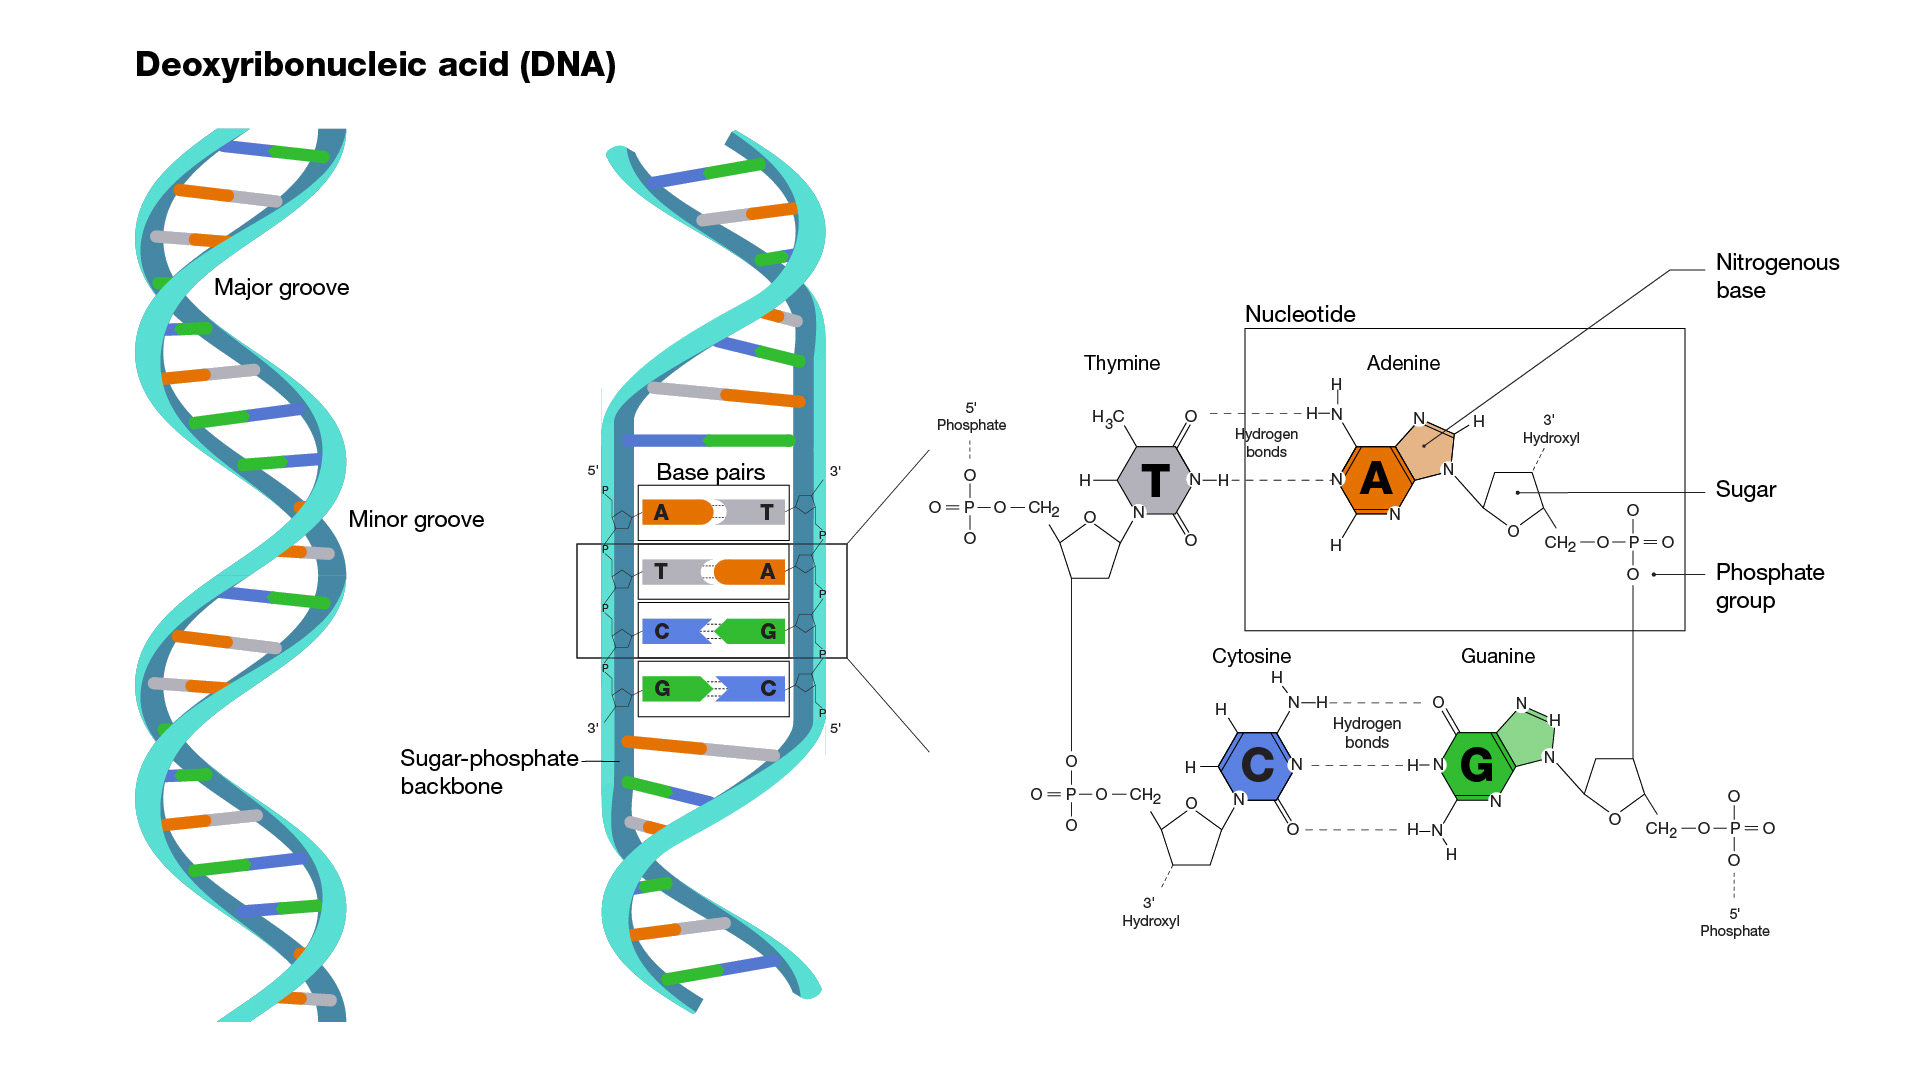
\includegraphics[width=0.6\textwidth]{resources/images/DNA-transparent.png}
  \caption{\textbf{A diagrammatic representation of the DNA} double helix structure along with detailed chemical structures of its components \cite{NHGRI2024-DNA}. On the right is the base pairing between nucleotides: specifically, adenine (A) binds with thymine (T), and cytosine (C) binds with guanine (G), all bound by hydrogen bonds.}
  \label{img:dna}
\end{figure}

\begin{wrapfigure}{l}{0.5\textwidth}  
  \centering
  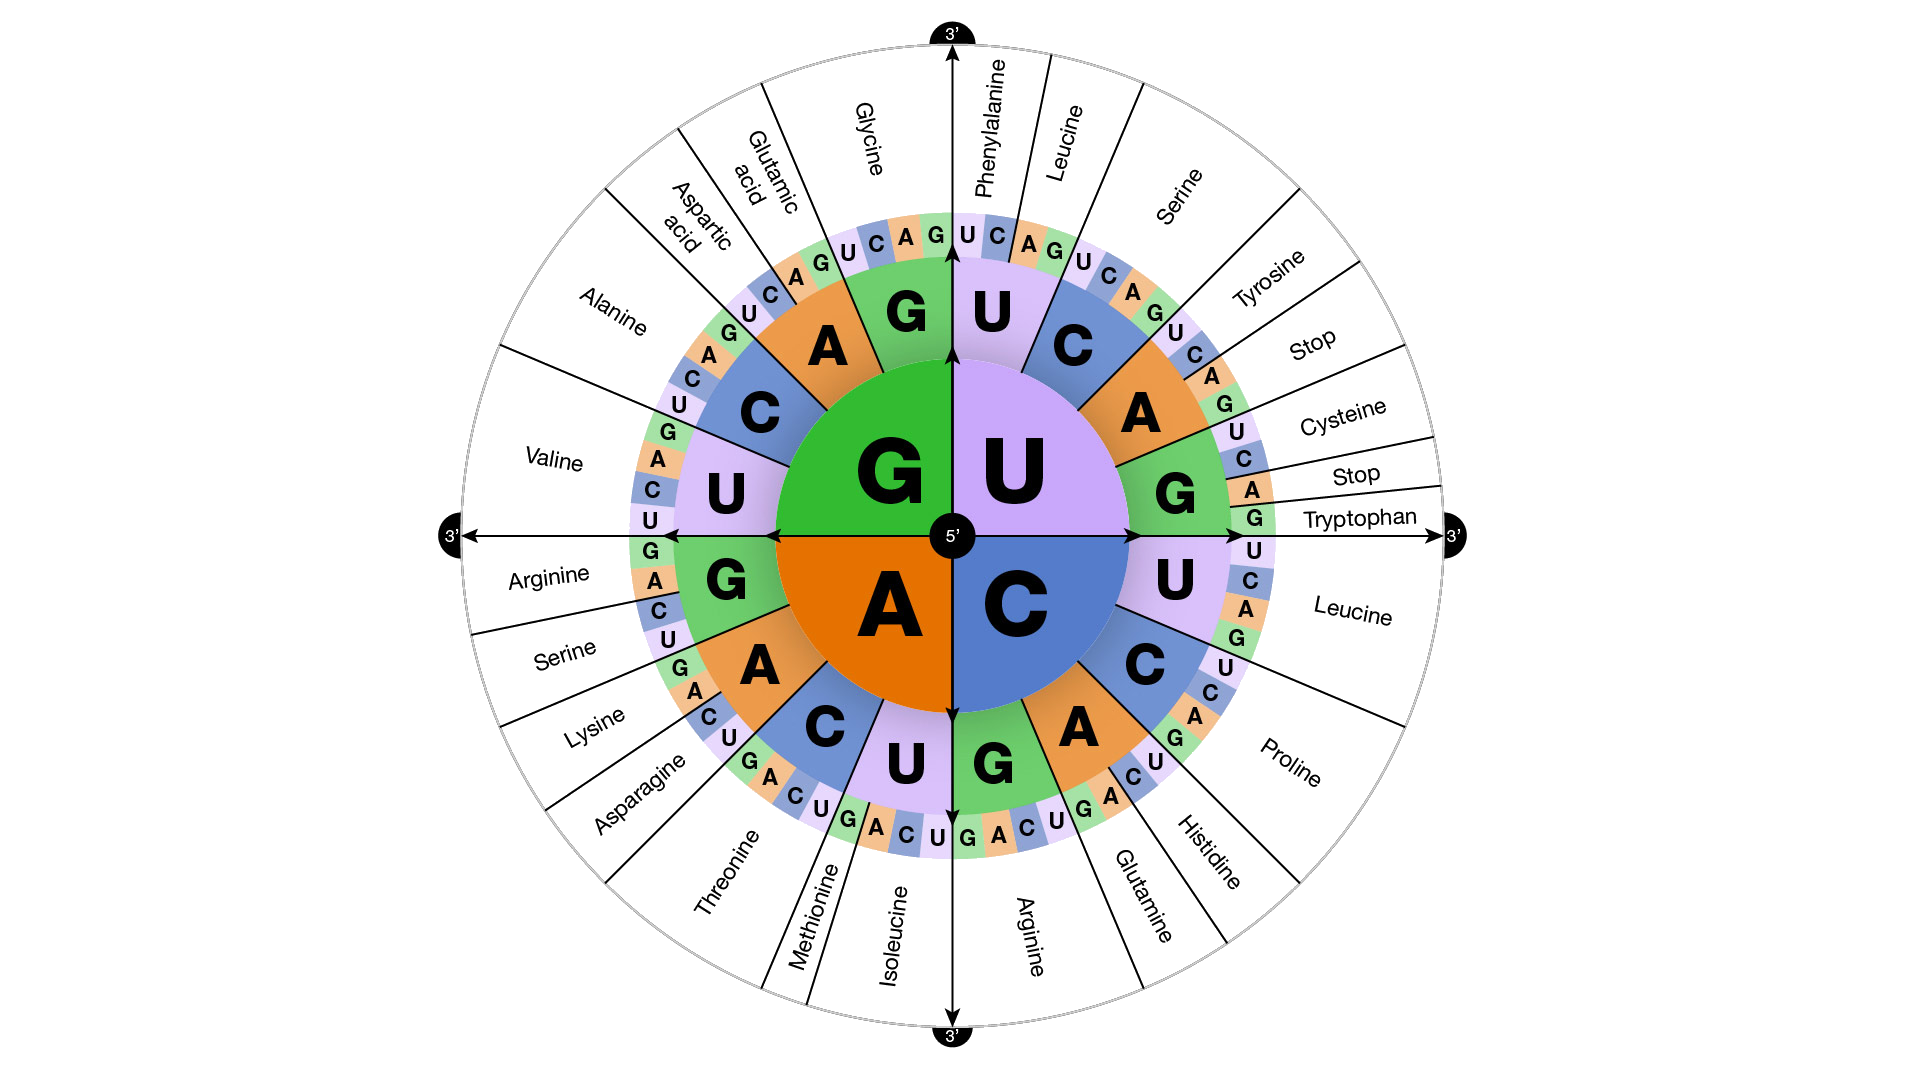
\includegraphics[width=0.48\textwidth]{resources/images/genetic-code.png} 
  \caption{\textbf{Genetic code}  \cite{NHGRI2024-Code} refers to the instructions contained in a gene that tell a cell how to make a specific protein. The code within each gene uses the four nucleotide bases of DNA — adenine (A), cytosine (C), guanine (G), and thymine (T) — in various ways to spell out three-letter “codons” that specify which amino acid is needed for each position within a protein.}
  \label{img:genetic-code}
\end{wrapfigure}

\gls{paired-end} (\autoref{img:pe-sequencing}), a technique used in \gls{ngs}, involves sequencing both ends of a \gls{dna} fragment to generate high-quality, alignable sequence data. This method allows for the \gls{sequencing} of both the forward and reverse ends of the fragments, providing two \gls{read}s per fragment. \gls{paired-end} is invaluable for detecting insertions, deletions, and rearrangements, and for improving the \gls{assembly} of complex \gls{genome}s. In the context of this research, \gls{paired-end} can enhance the resolution and accuracy of Mycobacterium tuberculosis genome assemblies by providing more information on the spatial relationships between \gls{dna} fragments, thus facilitating the identification of genomic variations and structural changes.

\begin{figure}[ht]
  \centering
  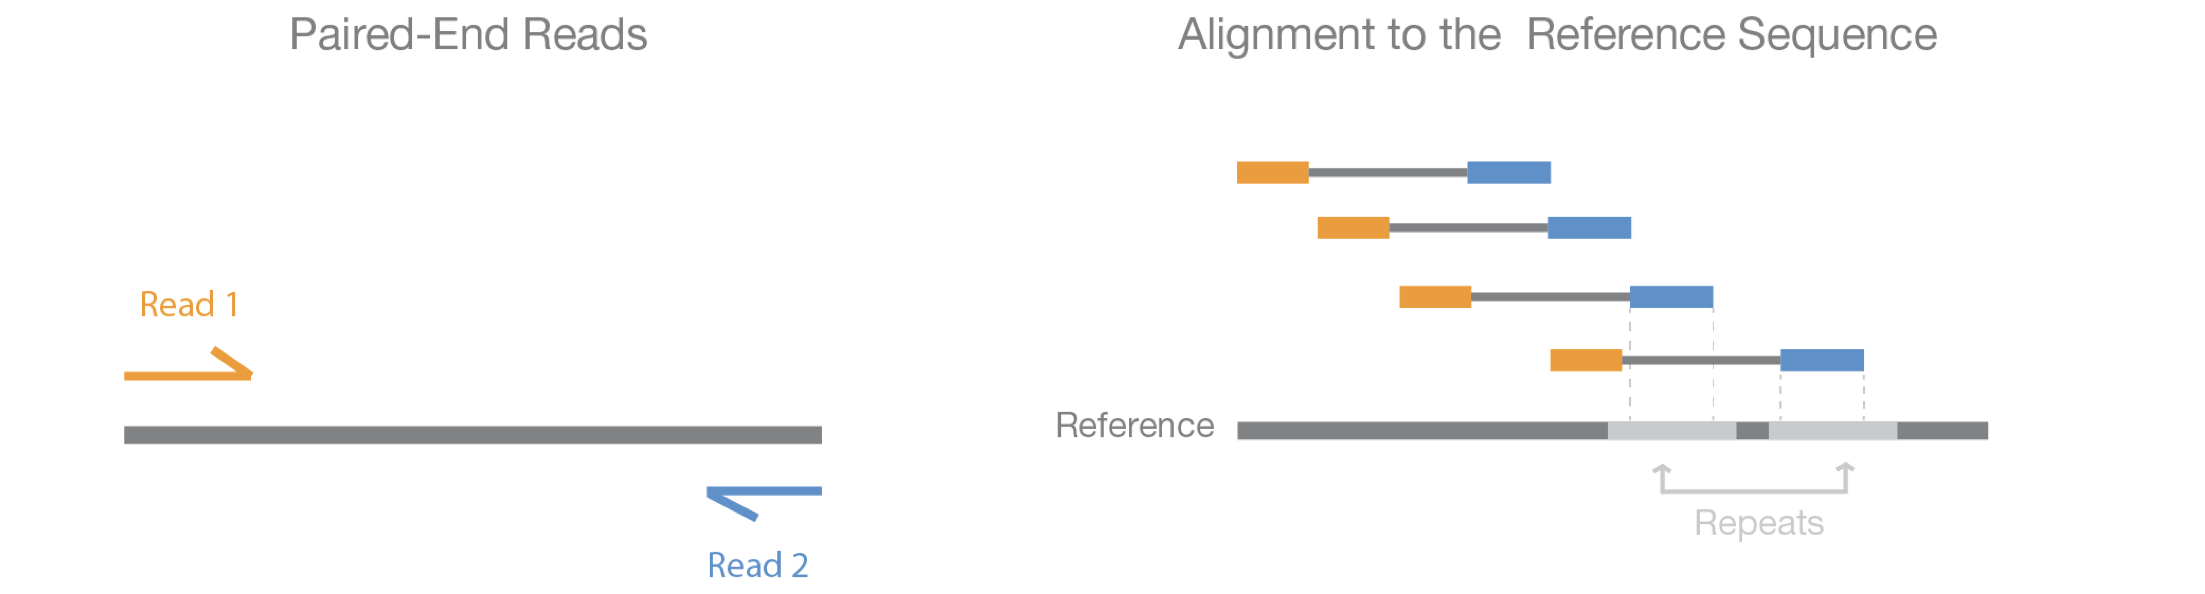
\includegraphics[width=\textwidth]{resources/images/paired-end (PE) sequencing.png}
  \caption{\textbf{Paired-End Sequencing and Alignment} \cite{Illumina2017-PE} — both ends of a DNA fragment are sequenced. The best advantage in this method is that since the distance between each paired-read is known, the alignment algorithms can able to use this information in-order to map the reads over repetitive regions more accurate. This results in better alignment of reads, especially across difficult-to-sequence, repetitive regions of the genome. Sequences aligned as read pairs allowing detection of indels that is not possible with single-read data.}
  \label{img:pe-sequencing}
\end{figure}

\section{Genome Assembly and Quality Assessment}

\begin{wrapfigure}{l}{0.5\textwidth}
  \centering
  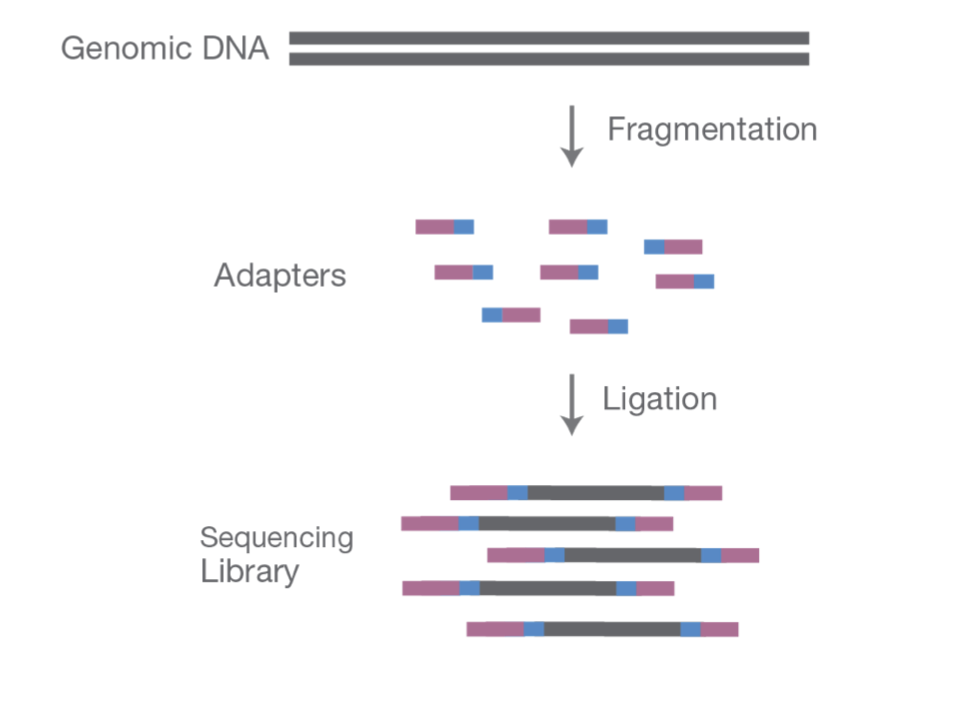
\includegraphics[width=0.48\textwidth]{resources/images/Library Preparation.png}
  \caption{\textbf{Library Preparation} \cite{Illumina2017-LP} — an illustration of the initial steps in preparing a Sequencing Library from genomic DNA. It is first fragmented into smaller pieces. Adapters (short, known DNA sequences) are then attached to the ends of these fragments. The adapters are used for several purposes, including the amplification of the fragments and as primer binding sites for Sequencing.}
  \label{img:library-preparation}
\end{wrapfigure}

\gls{ngs} is a high-throughput methodology that enables rapid \gls{sequencing} of the base pairs in \gls{dna} or RNA samples. \gls{ngs} has largely displaced older methods that were based on electrophoresis, as it is faster, more sensitive, and less expensive to operate. Thus, \gls{ngs} is now used in laboratories ranging from those focused on research on the history of life on Earth to those focused on identifying the exact genetic cause of an individual's disease. The \gls{ngs} workflow follows several key stages, including Library Preparation (\autoref{img:library-preparation}), Cluster Amplification (\autoref{img:cluster-amplification}), \gls{sequencing} (\autoref{img:sequencing}), and Alignment \& Analysis (\autoref{img:alignment-and-analysis}). At each stage the user's understanding of the nature and details of the genetics of an organism grows, from preparing the selected \gls{dna} or RNA sample in a usable \gls{fastq} \cite{Buffalo2015} to alignment of the \gls{ngs} \gls{read}s and analysis of the data. This process involves aligning and merging fragments from a longer \gls{dna} sequence, resulting in \gls{contig}s and \gls{scaffold}s. The quality of \gls{assembly} is paramount and can be assessed through various \gls{metrics}, such as \gls{n50}, \gls{n90}, \gls{l50}, \gls{l90}, \gls{total length}, \gls{gc}, \gls{largest contigs}, \gls{depth}, and the \gls{n's per 100 kbp}, which give insights into the size and completeness of the assembled \gls{genome}.

\begin{SCfigure}
  \centering
  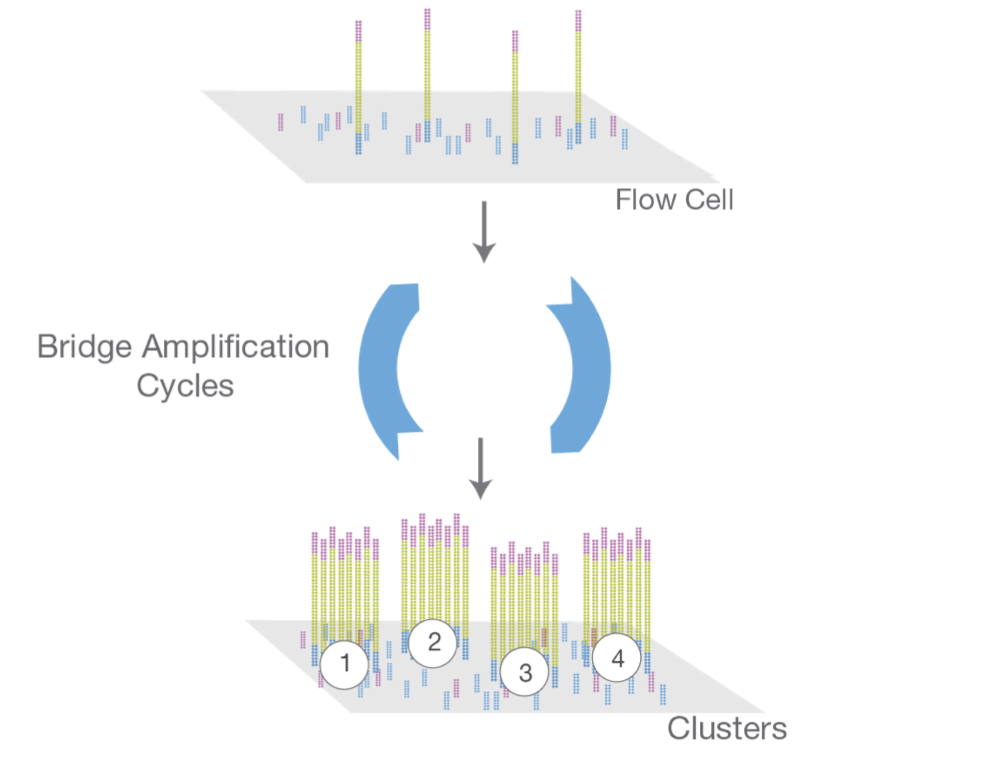
\includegraphics[width=0.48\textwidth]{resources/images/Cluster Amplification.png}
  \caption{\textbf{Cluster Amplification} \cite{Illumina2017-CA} — an image of the bridge amplification process, a crucial step in preparing DNA for sequencing on certain high-throughput platforms, such as Illumina Sequencing Systems. DNA fragments with adapters (blue and pink) ligated to their ends are attached to the flow cell surface (gold).}
  \label{img:cluster-amplification}
\end{SCfigure}

Every stage of high-throughput sequencing relies on robust and efficient methods to derive the \gls{dna} sequence. The first of these steps is the library preparation (\autoref{img:library-preparation}). Genomic \gls{dna} must be processed to be ready for \gls{sequencing}. It is fragmented down into small pieces. Adapters are then added to both ends of the fragments. Adapters are short, known \gls{dna} sequences. They have several functions. The first is that they form the priming site for the \gls{sequencing} Process to take place. The adapter also serves as the priming site for the amplification (\autoref{img:cluster-amplification}) of the \gls{dna}. The adapter can also contain a barcode, which allows for the pooling and identification of multiple samples within a single \gls{sequencing} Run.

\begin{SCfigure}
  \centering
  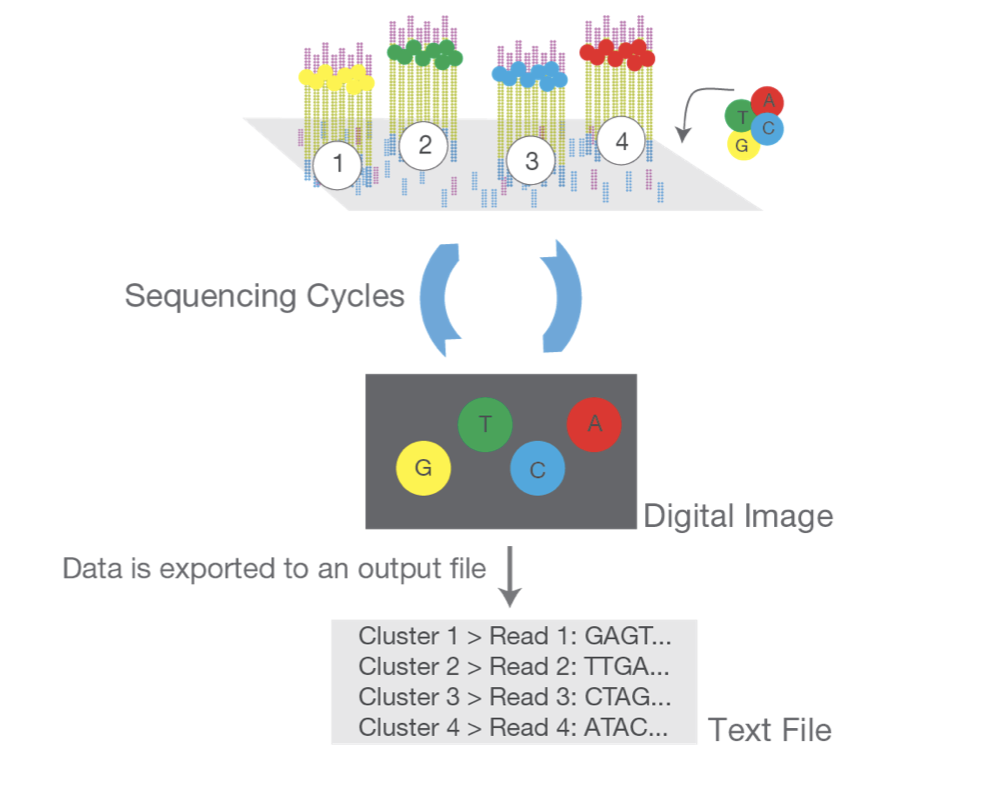
\includegraphics[width=0.48\textwidth]{resources/images/Sequencing.png}
  \caption{\textbf{Sequencing} \cite{Illumina2017-S} — each of the clusters generated from bridge amplification is sequenced one base at a time. A unique fluorescent signal is used to identify each of the four nucleotides (A, T, C, G). As the sequence is built, these signals are captured and translated into a digital image. That digital image is then converted into a text file containing the sequences of the DNA fragments.}
  \label{img:sequencing}
\end{SCfigure}

The library, now ready for attachment to a flow cell (\autoref{img:cluster-amplification}), will undergo clonal amplification on this glass slide. On the surface of the flow cell are lanes that are coated with oligonucleotides that are complementary to the adapters on the fragments. The library is loaded onto the flow cell where the fragments bind to the oligonucleotides. In bridge amplification the immobilized fragments will bend over and form a bridge and will fragment to oligonucleotides on the other strand. This bridge forms a localized clonal amplication site called a cluster. Within this cluster are many copies of that one DNA.


\begin{SCfigure}
  \centering
  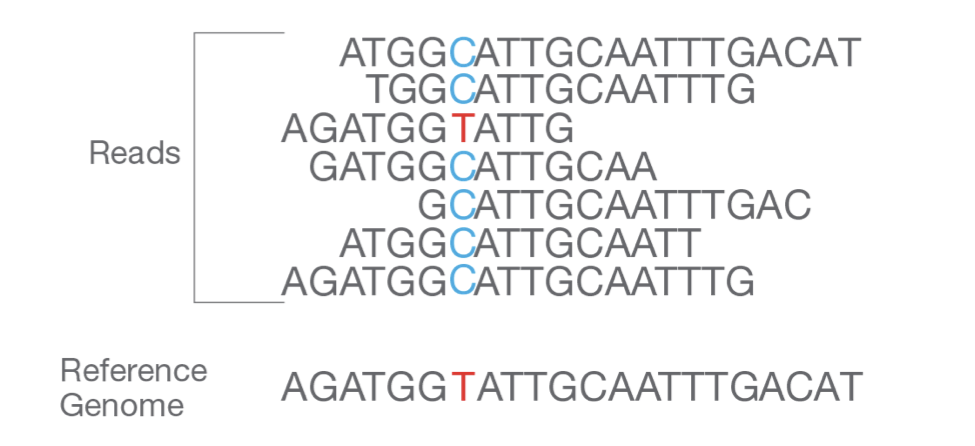
\includegraphics[width=0.48\textwidth]{resources/images/Alignment and Data Analysis.png}
  \caption{\textbf{Alignment \& Analysis} \cite{Illumina2017-ADA} — short DNA sequences (Reads) are matched against a longer ‘Reference Genome’ sequence. The highlighted sections in the Reads indicate a match, or mismatch, to the Reference Sequence.}
  \label{img:alignment-and-analysis}
\end{SCfigure}

The actual \gls{sequencing} (\autoref{img:sequencing}) occurs through a series of cycles. Each cycle adds one nucleotide at a time to the \gls{dna} strand. The nucleotide, or base, is read by a fluorescent signal; the signal is captured and recorded. In this way chemical information is translated to digital data (each of the four \gls{dna} bases is associated with a unique color). The process cycles, building a sequence read that is complementary to the \gls{dna} template in the library.

Resulting sequence reads are computationally aligned to a Reference \gls{genome} (\autoref{img:alignment-and-analysis}); this process identifies where in the \gls{genome} each \gls{read} comes from and is critical for variant detection and understanding the structure of the \gls{genome}. Additionally, \gls{read}s are assessed for quality; each base call is assigned a quality score, which reflects the confidence of the base call. Ultimately, each analysis reveals variations and mutations, information about genetic predisposition to diseases, and much more.

\section{Impact of Trimming on Assembly Metrics}

\gls{trimming} in \gls{ngs} is a crucial pre-processing step. During this process, low-quality bases and adapter sequences are carefully removed from \gls{read}s. This significantly affects the quality of the subsequent \gls{assembly}. The effectiveness of different \gls{trimming} Methods \cite{fastp}, such as adapter trimming, quality trimming, and sliding window trimming, can be evaluated based on their impact on important \gls{metrics} like \gls{n50}, \gls{gc} content, and error rates. These techniques are essential to ensure that only high-quality \gls{read}s advance to the \gls{assembly} phase, enhancing the overall accuracy and reliability of genomic analysis.

Moreover, the selection of a \gls{trimming} Method can significantly influence downstream analysis and interpretation of \gls{ngs} data. For instance, quality trimming, which focuses on removing bases with low-quality scores, can markedly decrease false positives in variant calling. Conversely, adapter trimming is vital for avoiding artificial chimeras and ensuring the assembly of genuine genomic sequences. The complexities of these methods underscore the importance of a well-thought-out \gls{trimming} Strategy, customized to the specific needs of each \gls{ngs} project, to achieve the best results in Genomic \gls{sequencing} and Analysis.

\section{Data Visualization in Genomic Assembly Analysis}

Data Visualization \cite{Chen2007} plays a crucial role in understanding and interpreting the vast amount of data generated by \gls{ngs}.  Visualization tools such as \gls{heatmap}s, \gls{bar}, and \gls{scatter}s can be used to represent various aspects of \gls{assembly} and \gls{trimming} efficiency. For instance, \gls{heatmap}s can illustrate the \gls{deviation} in \gls{read} quality before and after \gls{trimming}, while \gls{bar} can show the relationship between trimming methods and key \gls{metrics} like \gls{n50} and \gls{n's per 100 kbp} \cite{quast}.

\section{Conclusion}

In summary, \gls{ngs} and its associated data analysis techniques, including \gls{trimming} and Data Visualization, are crucial in assessing \gls{assembly} Quality \cite{Wang2022}. Understanding these concepts, as underlined in the recommended literature, provides vital insights into genomic studies, paving the way for advancements in genetics and beyond.
 \clearpage
\chapter{Pipeline Design and Execution}

The \gls{ngs}-pipeline represents a comprehensive solution for \gls{ngs} data analysis, designed to streamline the process of \gls{trimming}, \gls{genome} Assembly, and \gls{assembly} Quality Assessment. By integrating advanced bioinformatics tools such as fastp for \gls{trimming}, SPAdes for \gls{assembly}, and QUAST for Quality Evaluation, this pipeline ensures high fidelity in data processing and analysis. The entire codebase of the \gls{ngs}-pipeline is openly accessible at \url{https://github.com/shliamin/NGS-pipeline/blob/main/main.nf}, facilitating its adoption and customization for diverse research needs.

\section{Data Foundation}

\subsection{Input Data}
The data for the analysis were sourced from the publicly available Sequence \gls{read} Archive (SRA) at the National Center for Biotechnology Information (NCBI). Due to technical constraints and to ensure compatibility with the computing environment, it was decided to directly install SRA-Tools for command-line usage.

The procedure for downloading SRA-formatted data involved the use of the \texttt{prefetch} command, followed by conversion to \gls{fastq} using \texttt{fasterq-dump}, with the \texttt{--split-3} option employed for processing Paired-End \gls{read}s. For instance, to obtain data for Paired Genomic \gls{dna} Sequencing Analysis, the following commands were executed:
\begin{verbatim}
./prefetch SRR26630744
./fasterq-dump --split-3 SRR26630744
\end{verbatim}

This process successfully produced the necessary files for the analysis of paired genomic \gls{sequencing}: \texttt{SRR26630744\_1.fastq} and \texttt{SRR26630744\_2.fastq}. This approach requires \gls{read}s from both ends of a \gls{dna} fragment, a technique referred to as \gls{paired-end}. Typically, \gls{paired-end} involves two files, each containing \gls{read}s from one end of the fragment. This data was then consistently used for each run of the software pipeline and testing of different methods of \gls{trimming}, thus producing consistent results within the scientific method of research.


\subsection{Data Preprocessing}

Data preprocessing is a critical step in the pipeline, aimed at improving the quality of the input data for subsequent analyses. The preprocessing includes Quality \gls{trimming}, Sliding Window \gls{trimming}, Adapter Removal, Length Filtering, and Complexity Filtering as well as their hybrids with different parameters. These steps are executed using fastp, chosen for its versatility and high performance. The process not only reduces the computational load by removing low-quality sequences but also enhances the reliability of \gls{genome} Assemblies by reducing the number of regions of the \gls{genome} whose sequence is unknown or uncertain in a given context.



\section{Software Utilized}

This section details the computational tools and software (\autoref{table:software}) utilized in the pipeline. Each tool was selected based on its efficiency, accuracy, and compatibility with the overall design of the pipeline. The versions of the software are specified to ensure reproducibility and consistency of the analysis. The following table summarizes the software tools and their respective versions used:

\begin{table}[ht]
\centering
\begin{tabular}{l l}
\hline
\textbf{Software} & \textbf{Version} \\ \hline
Nextflow & 23.10.0 \\
fastp & 0.23.4 \\
SPAdes & 3.15.5 \\
QUAST & 5.2.0 \\ \hline
\end{tabular}
\caption{Summary of software tools and versions used in the pipeline.}
\label{table:software}
\end{table}

\subsection{fastp for Trimming}

\textit{fastp} is utilized within our pipeline for its efficiency in \gls{trimming} low-quality bases and removing adapters from raw sequencing reads. The tool's versatility allows for the execution of a variety of \gls{trimming} Combinations, enhancing the quality of data for downstream analysis. The \gls{trimming} combinations implemented are described below:

\paragraph{\gls{trimming} Combinations:}
The \gls{trimming} Combinations, such as \textit{QualityTrim\_Q25} and \textit{AdapterTrim\_Q25}, employ a systematic approach that combines the \gls{trimming} Type with specific parameters, delineated by underscores (\_). Initially, five basic \gls{trimming} Methods (\autoref{table:basic_trimming_methods}) with averaged parameters are applied, addressing various potential issues in sequencing data:

\begin{itemize}
    \item \textbf{Quality Trimming:} Removes regions with low sequencing quality to improve downstream analysis accuracy.
    \item \textbf{Adapter Trimming:} Excises adapter sequences to prevent interference in read alignment and analysis.
    \item \textbf{Length Filtering:} Retains reads of specified lengths, essential for analyses like assembly.
    \item \textbf{Complexity Filtering:} Eliminates low complexity sequences that may be repetitive or non-informative.
    \item \textbf{Sliding Window Trimming:} Conducts quality trimming within a sliding window, balancing quality control and data retention.
\end{itemize}

\paragraph{Parameters:}
Parameters follow the \gls{trimming} Type, indicated by a prefix (e.g., \textit{Q25} for a quality threshold of 25, \textit{75} for length filtering at 75 bases). 

\paragraph{Hybrids:}
Hybrid combinations (\autoref{table:hybrid_trimming_methods}) , such as \textit{QualityAdapterHybrid\_Q25}, integrate two \gls{trimming} Methods, providing a versatile approach to data preprocessing. In the initial run of the pipeline we explore 16 distinct \gls{trimming} Methods, including a \textit{NoTrimming} option to assess the impact of preprocessing on data quality.

The naming consistency across these combinations plays a critical role in the pipeline's execution, allowing for traceability of data from input through to the final output. This systematic approach facilitates reproducibility and understanding of the pipeline's workflow, enabling researchers and future users to modify or extend the pipeline with ease.

\paragraph{Demonstration of Naming Consistency:}
The logical and transparent naming conventions ensure each data piece can be followed through the pipeline, maintaining the integrity of the workflow and simplifying the reproduction of results.

\begin{figure}[H]
    \centering
    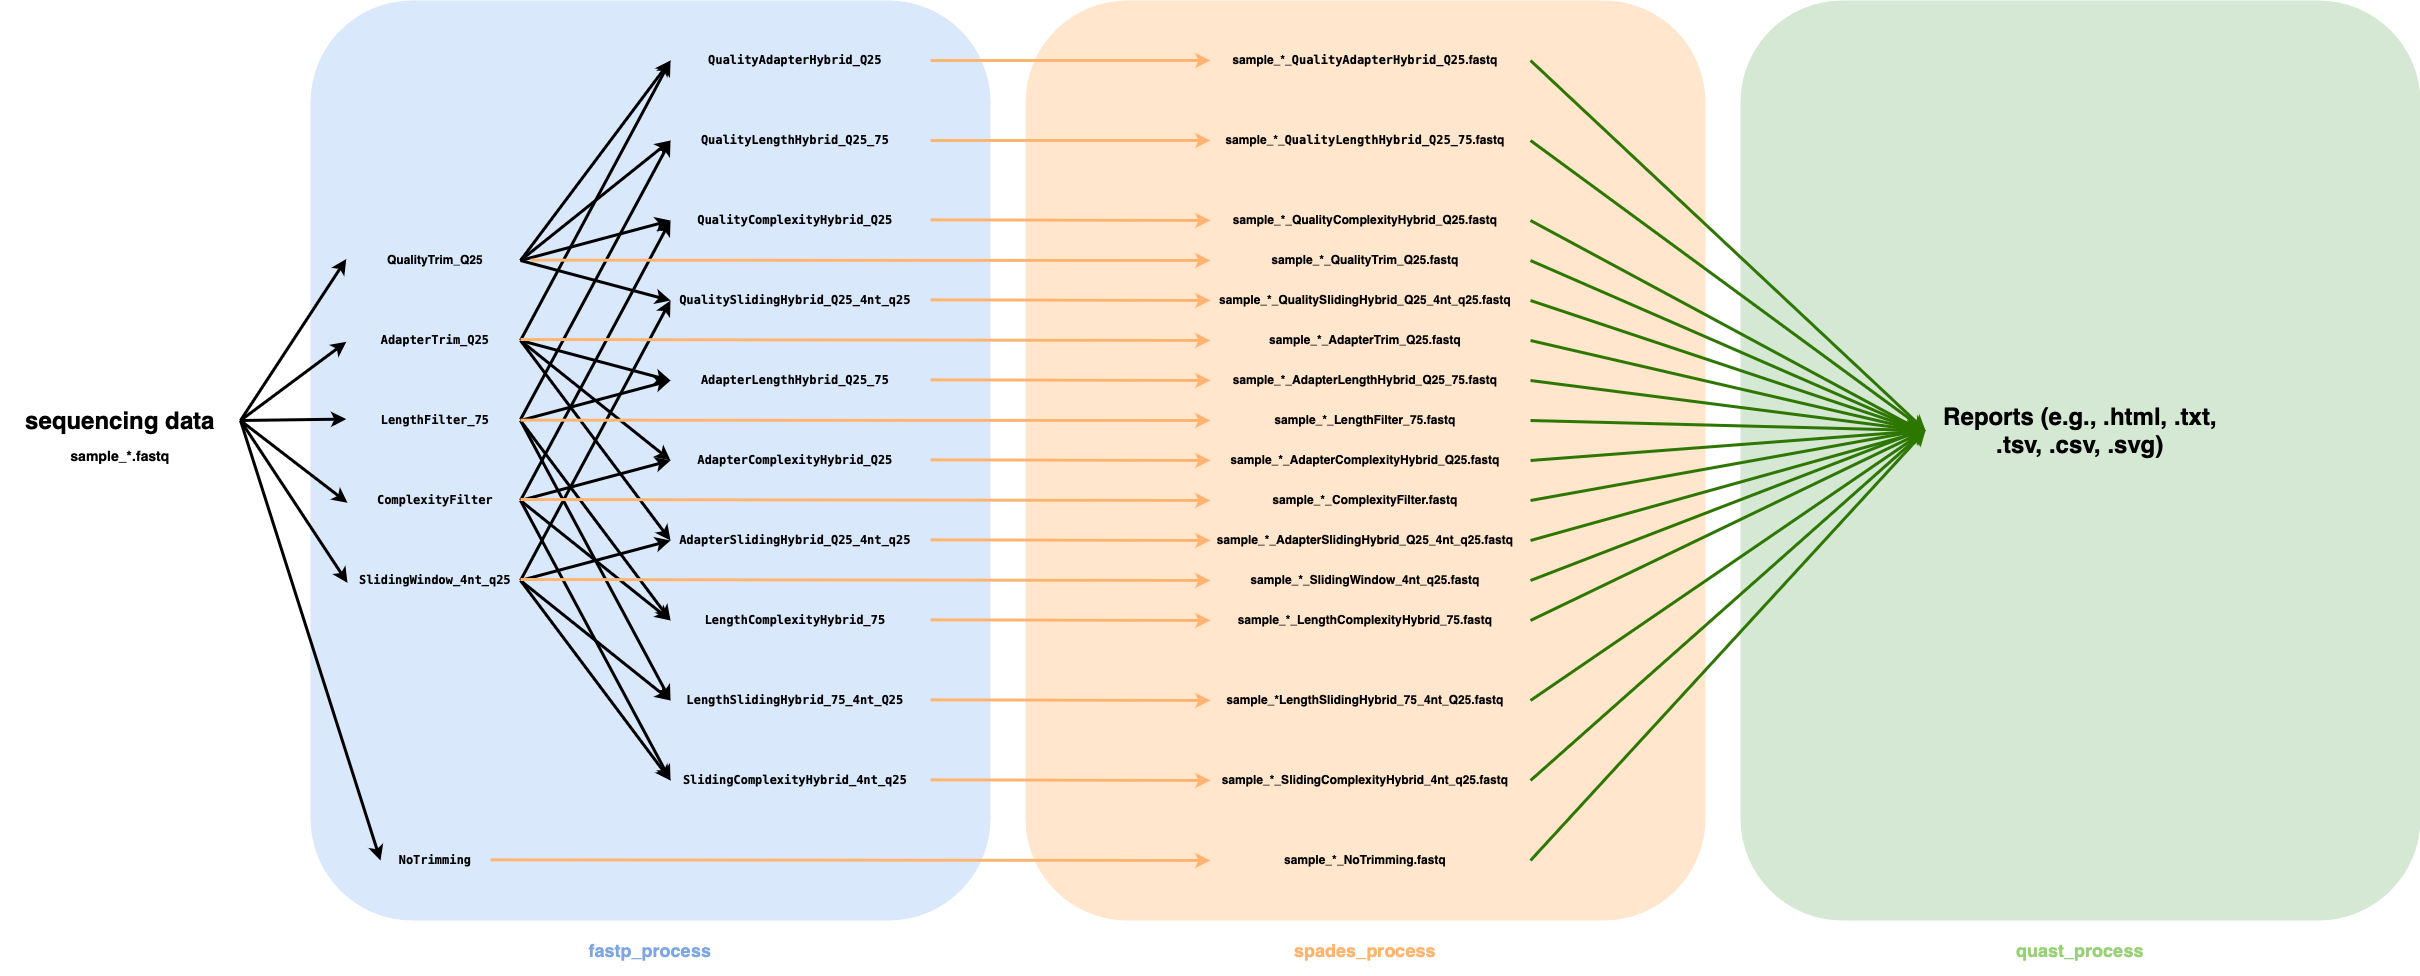
\includegraphics[width=\textwidth]{resources/images/NGS-pipeline.drawio.png}
    \caption{\textbf{Schematic representation of the data flow through the \gls{trimming}, Assembling and Evaluating stages of the software pipeline}. Each \gls{trimming} Method is systematically named to reflect the method and parameters used, ensuring traceability and clarity of the data processing steps.}
    \label{fig:trimming_pipeline}
\end{figure}

The \autoref{fig:trimming_pipeline} illustrates the systematic approach to \gls{trimming}, showcasing the various combinations of methods and their corresponding parameters. This naming consistency allows for each piece of data to be traced through the pipeline, ensuring that the process from initial input to final output, including all intermediate steps, is clear and reproducible.

\paragraph{\gls{trimming} Methods with their Parameters and Expected Outcomes:}

In the initial run of the pipeline, various \gls{trimming} Methods (\autoref{table:basic_trimming_methods} and \autoref{table:hybrid_trimming_methods}) are employed to ensure the highest quality of the sequence data. The table below (\autoref{table:basic_trimming_methods}) summarize the 5 Basic \gls{trimming} Methods, their descriptions, and the expected outcomes upon processing:

\begin{table}[H]
\centering
\begin{tabular}{p{0.2\linewidth} p{0.4\linewidth} p{0.3\linewidth}}
\hline
\textbf{Trimming Method} & \textbf{Description} & \textbf{Expected Result} \\ \hline
NoTrimming & No trimming applied. & Unaltered data \\
QualityTrim\_Q25 & Trims low-quality bases below Q25. & Higher quality \\
AdapterTrim\_Q25 & Removes adapter sequences. & No adapters \\
LengthFilter\_75 & Excludes reads below 75 bases. & Consistent length \\
ComplexityFilter & Filters low complexity sequences. & Reduced complexity \\
SlidingWindow\newline\_4nt\_q25 & Sliding window quality trimming: 4nt window, q25 cutoff & Balanced quality \\
\hline
\end{tabular}
\caption{Basic Trimming Methods in the initial run of the pipeline.}
\label{table:basic_trimming_methods}
\end{table}

Each method is designed to address specific types of artifacts within the sequencing data. The selection of \gls{trimming} Method is crucial to prepare the dataset for accurate assembly and analysis. The most averaged parameters were chosen for each \gls{trimming} Method.

\begin{table}[H]
\centering
\begin{tabular}{l l}
\hline
\textbf{Trimming Method} & \textbf{Expected Result} \\ \hline
QualitySlidingHybrid\_Q25\_4nt\_q25 & Enhanced quality \\
QualityAdapterHybrid\_Q25 & Clean reads \\
LengthComplexityHybrid\_75 & Lengthy, non-repetitive \\
SlidingComplexityHybrid\_4nt\_q25 & Quality, non-repetitive \\
AdapterSlidingHybrid\_Q25\_4nt\_q25 & No adapters, balanced \\
QualityLengthHybrid\_Q25\_75 & High quality, uniform \\
QualityComplexityHybrid\_Q25 & High quality, unique \\
AdapterLengthHybrid\_Q25\_75 & No adapters, consistent \\
AdapterComplexityHybrid\_Q25 & No adapters, unique \\
LengthSlidingHybrid\_75\_4nt\_Q25 & Uniform length, balanced \\
\hline
\end{tabular}
\caption{Hybrid Trimming Methods in the initial run of the pipeline.}
\label{table:hybrid_trimming_methods}
\end{table}

The hybrid \gls{trimming} Methods (\autoref{table:hybrid_trimming_methods}) implemented in the pipeline are the result of combinations without repetitions of the 5 Basic \gls{trimming} Methods. Given 5 Basic \gls{trimming} Methods, the number of unique hybrid combinations that can be created without repeating any single method can be calculated using the formula for combinations without repetition, also known as binomial coefficients. This is mathematically represented as:

\[
C(n, k) = \frac{n!}{k!(n-k)!}
\]

For our case, with \( n = 5 \) basic methods and \( k = 2 \) methods per combination, the formula simplifies to:

\[
C(5, 2) = \frac{5!}{2!(5-2)!} = \frac{5 \times 4}{2 \times 1} = 10
\]

This combinatorial approach yields exactly 10 unique hybrid methods, which are then utilized in the first run of the software pipeline to ensure a comprehensive exploration of \gls{trimming} Effects. That is the reason for choosing exactly 16 \gls{trimming} Methods (10+5+1), including the NoTrimming Method, for the first run of the software pipeline.

\paragraph{The fastp\_process:}

Within the pipeline, the `fastp\_process` is designated to perform Sequence \gls{trimming} and Quality Control. This process is initiated with a unique label and dynamically assigned tags based on \gls{trimming} Parameters and input file names. The input section specifies a tuple consisting of \gls{trimming} Parameters and associated \gls{read} files. The output is similarly structured, producing a tuple that includes the original \gls{trimming} Parameters and paths to the trimmed \gls{fastq} files. It takes \gls{paired-end} \gls{read}s and the \gls{trimming} Parameters as input and generates trimmed sequence files based on the specified parameters. The process dynamically constructs the fastp command based on the \gls{trimming} Method provided, applying the relevant \gls{trimming} Options.

Below is the code to the \textit{fastp\_process}, which is divided into 2 parts (\autoref{lst:fastp} and \autoref{lst:trimming_params_handling}) for ease of reading, in which only essential parts of it are indicated, the rest of the points are commented out for brevity.


\begin{lstlisting}[language=Java, , label={lst:fastp}, caption={Comprehensive Overview of the fastp\_process in the NGS Pipeline.}]
process fastp_process {
    label 'fastp'
    tag "${trimParams}_${reads[0].getName()}"

    input:
        tuple val(trimParams), file(reads)

    output:
        tuple val(trimParams), \
        path("${reads[0].simpleName}_${trimParams}.fastq"), \
        path("${reads[1].simpleName}_${trimParams}.fastq")

    script:
        String trimParamsStr = trimParams.toString().trim()
        def fastpCmd = "fastp --in1 ${reads[0]} --in2 ${reads[1]}"
        String outputFileName1 = "${reads[0].simpleName}_${trimParams}.fastq"
        String outputFileName2 = "${reads[1].simpleName}_${trimParams}.fastq"
        fastpCmd += " --out1 ${outputFileName1} --out2 ${outputFileName2}"
        String htmlReport = "${reads[0].simpleName}_${trimParams}.html"
        String jsonReport = "${reads[0].simpleName}_${trimParams}.json"
        fastpCmd += " --html ${htmlReport} --json ${jsonReport}"

        // Representation of dynamic trimming parameters handling (omitted for brevity)
        // def trimActionMap = [...]
        // trimActionMap.each { key, action -> ... }

        """
        set -euo pipefail
        echo "Trimming parameters: ${trimParams}"
        if [ ${reads.size()} -ne 2 ]; then
            echo "Error: Expected two reads files, but got ${reads.size()}"
            exit 1
        fi
        ${fastpCmd}
        echo "fastp process for ${trimParams}_${reads[0].getName()} completed successfully."
        """
}
\end{lstlisting}

This \autoref{lst:fastp} highlights the input and output file handling, command construction, and application of \gls{trimming} Parameters as part of the \texttt{fastp} command execution within the pipeline. The iterative structure ensures that the appropriate action is taken for each set of \gls{trimming} Parameters. The robustness of the script is evidenced by error handling that checks for the expected pair of \gls{read} files, ensuring data integrity. Upon successful execution, the process concludes with an informative message indicating the completion of the `fastp` operation for the given parameters.

The core of the `fastp\_process` lies in its script section (\autoref{lst:trimming_params_handling}), which constructs the `fastp` command with parameters tailored to the \gls{trimming} Requirements. Here, the \gls{trimming} Parameters are parsed and translated into `fastp` command options. A mapping structure, `trimActionMap`, is defined to convert symbolic \gls{trimming} Names into their respective `fastp` command-line arguments. This approach ensures that each \gls{trimming} Method is applied correctly based on the input data characteristics. 


\begin{lstlisting}[language=Java, , label={lst:trimming_params_handling}, caption={Representation of dynamic trimming parameters handling}]
def parts = trimParamsStr.tokenize('_')

    def trimActionMap = [
    QualityTrim: { String q -> 
      "--qualified_quality_phred ${q.replace('Q', '')}" 
    },
    AdapterTrim: { String q -> 
      "--detect_adapter_for_pe --qualified_quality_phred " +
      "${q.replace('Q', '')}" 
    },
    
    // The rest of the trimming methods that are omitted for brevity
    
    NoTrimming: { _ -> 
      "--disable_adapter_trimming --disable_quality_filtering " +
      "--disable_length_filtering" 
    }
    ]

    trimActionMap.each { key, action ->
    if (trimParamsStr.startsWith(key)) {
        fastpCmd += " " + action(parts.drop(1))
        return
      }
    }
\end{lstlisting}

For example, based on the \gls{trimming} Method "QualityTrim\_Q25" a fastp command will be dynamically created (\autoref{lst:trimming_params_handling}) with the parameter "-qualified\_quality\_phred" and the quality value 25 will be automatically added (the numbers are also dynamically set) means phred quality >=Q25 is qualified. In this example a quality value of 25 corresponds to an error probability of 1 in 100 (i.e., 99\% accuracy), which is a fairly high threshold for many bioinformatics and genomics applications.


Different combinations (\autoref{tab:phred_scores}) of \gls{sequencing} quality parameters (Phred-Score Q) such as Q15, Q20, Q25, and Q30 are presented within this work. These parameters are used to provide varying degrees of rigor in \gls{trimming} \gls{read}s, allowing the data cleaning process to be customized for specific study purposes.

\begin{table}[ht]
\centering
\begin{tabular}{cc}
\hline
\textbf{Phred-Score Q} & \textbf{Accurancy (\%)} \\
\hline
Q15 & 99.97\% \\
Q20 & 99.99\% \\
Q25 & 99.999\% \\
Q30 & 99.9999\% \\
\end{tabular}
\caption{Correlation between Phred-Score Q and percentage accuracy.}
\label{tab:phred_scores}
\end{table}




\subsection{SPAdes for Genome Assembly}
For the \gls{assembly} stage, \textit{SPAdes} (St. Petersburg genome assembler) was chosen for its versatility and effectiveness in assembling high-quality \gls{genome}s from \gls{ngs} data coming from the preceding \texttt{fastp\_process} (\autoref{lst:fastp}). In our project, \textit{SPAdes} was employed to construct high-quality genomic assemblies from the preprocessed \gls{read}s. The assembler's advanced algorithms enable the reconstruction of genomic sequences with high accuracy, making it an indispensable tool for our software pipeline.

\paragraph{The spades\_process:}

The \autoref{lst:spades}represents the \texttt{spades\_process} within the Nextflow pipeline, aimed at conducting \gls{assembly} utilizing the SPAdes Software. This process is integral to transforming Sequencing \gls{read}s into Assembled \gls{genome}s, a crucial step in understanding the genomic architecture of the organism under study.

\begin{lstlisting}[language=Java, label={lst:spades}, caption={SPAdes genome assembly process in Nextflow.}]
process spades_process {
  label 'spades'
  tag "${trimParams}"

  input:
    tuple val(trimParams), path(read1), path(read2)
    
  output:
    path "scaffolds_${trimParams}.fasta"

  cpus 4
  memory '8 GB'

  script:
    """
    set -euo pipefail
    echo "Read1: ${read1}"
    echo "Read2: ${read2}"
    echo "Starting SPAdes genome assembly for ${trimParams}..."
    spades.py --isolate -1 ${read1} -2 ${read2} -o output_${trimParams}
    mv output_${trimParams}/scaffolds.fasta scaffolds_${trimParams}.fasta
    echo "SPAdes genome assembly for ${trimParams} completed successfully."
    """
}
\end{lstlisting}

\textbf{Key Components of the \autoref{lst:spades}:}

\begin{itemize}
    \item \textbf{Label and Tag:} The process is labeled 'spades' and tagged with \gls{trimming} Parameters, facilitating resource allocation and identification of the process's tasks.
    \item \textbf{Input:} Accepts a tuple comprising \gls{trimming} Parameters and paths to paired-end \gls{read} files, signifying the raw data for \gls{assembly}.
    \item \textbf{Output:} Produces a FASTA file named after the \gls{trimming} Parameters, containing the assembled \gls{scaffold}s, which are the result of the SPAdes assembly process.
    \item \textbf{Resources:} Allocated with 4 CPUs and 8 GB of memory, ensuring sufficient computational resources for the assembly task. (This parameter can be adjusted to suit the needs and power of the computer individually. This demonstrates the parameters used in this study.)
    \item \textbf{Script:} Executes the SPAdes command with the provided \gls{read}s, outputting the \gls{assembly} into a designated folder, subsequently moving the \gls{scaffold}s file to a specified path. The use of \texttt{set -euo pipefail} parameter ensures that the script will stop if errors occur, which increases the reliability of the process execution.
\end{itemize}

This process exemplifies a critical step (\autoref{lst:spades}) in the software pipeline, converting Trimmed Sequencing \gls{read}s into a coherent genomic structure, thereby enabling further genomic analyses.


\subsection{QUAST for Quality Assessment}
Upon completion of the \gls{assembly}, \textit{QUAST} (Quality Assessment Tool for Genome Assemblies) was utilized to evaluate the quality of the assembled sequences. \textit{QUAST} provides comprehensive Quality \gls{metrics}, including contiguity, coverage, and correctness of the assemblies. By applying \textit{QUAST}, we were able to assess the assembly quality in a quantitative manner, allowing for the identification and correction of potential errors in the \autoref{lst:spades} Assembled \gls{genome}s. This quality assessment step is crucial for ensuring that the final genomic sequences are accurate and suitable for downstream analyses.

\paragraph{The quast\_process:}

described below (\autoref{lst:quast}), is an important component of the software pipeline designed to evaluate genomic assemblies derived from the previous \texttt{spades\_process} using QUAST. This process facilitates \gls{assembly} Quality Assessment by providing critical insight into the integrity and completeness of Assembled \gls{genome}s. This creates reports on each \gls{genome} collected here, which we then analyze. Different file extensions are available to choose from, e.g. TSV, which we use in further analysis.

\begin{lstlisting}[language=Java, label={lst:quast}, caption={QUAST quality assessment process in Nextflow.}]
process quast_process {

  input:
    path genomes

  output:
    path "reports"

  script:
    """
    mkdir -p reports
    set -euo pipefail
    for genome in ${genomes}
    do
      genome_name=\$(basename \$genome .fasta)
      echo "Starting QUAST quality assessment for \$genome_name..."
      quast.py -o reports/output_\${genome_name} \${genome}
      mv reports/output_\${genome_name}/report.html \
        reports/report_\${genome_name}.html
      echo "QUAST quality assessment for \$genome_name completed."
    done
    """
}
\end{lstlisting}

\textbf{Key Elements of the \autoref{lst:quast}:}

\begin{itemize}
    \item \textbf{Input:} It accepts a path to \gls{genome} Assemblies, serving as the input for the quality assessment procedure.
    \item \textbf{Output:} Generates a directory named "reports" which will contain HTML reports for each Analyzed \gls{genome}, summarizing the quality assessment results.
    \item \textbf{Script:} This segment of the process encapsulates the commands for executing QUAST on each \gls{assembly}, highlighting the iterative approach to generate comprehensive quality reports. The use of a loop to process multiple \gls{genome}s and the subsequent organization of reports demonstrate the process's capability to handle batch assessments, making it a scalable solution for quality analysis.
\end{itemize}

Overall, \texttt{quast\_process} (\autoref{lst:quast}) represents an important step towards ensuring the reliability of genomic assemblies by offering a systematic approach to quality control in genomic research.













\section{Pipeline Implementation}

\subsection{Initial Setup in Nextflow}

The provided \autoref{lst:initial} is a crucial component of a Nextflow pipeline designed for processing \gls{ngs} data. This segment outlines the initial setup for data preprocessing, specifically focusing on the diversity of \gls{trimming} Methods applied prior to \gls{assembly} and Quality Assessment.

\begin{lstlisting}[language=Java, label={lst:initial}, caption={Initial setup and trimming strategy definition in Nextflow.}]
// Define input and output directory parameters
params.input_dir = 'raw_data'

// Define a list of different trimming combinations for sequence processing
def trimmingCombinations = [
  "QualityTrim_Q25",
  "AdapterTrim_Q25",
  "LengthFilter_75",
  "ComplexityFilter",
  "SlidingWindow_4nt_q25",
  "QualitySlidingHybrid_Q25_4nt_q25", // QualityTrim_Q25 + SlidingWindow_4nt_q25
  // Other trimming combinations
  "NoTrimming"
]

/* Create a channel with trimming combinations 
  and pair them with file pairs from the input directory
*/
Channel
  .from(trimmingCombinations)
  .combine(Channel.fromFilePairs("${params.input_dir}/*_{1,2}.fastq"))
  .map { trimParams, sampleId, files -> 
    println("Trim Params: ${trimParams}, Files: ${files}") 
    tuple(trimParams, files) 
  }
  .set { trimmingChannel }

\end{lstlisting}

\textbf{Key Elements of the \autoref{lst:initial}:}

\begin{itemize}
    \item \textbf{Parameter Definition:} The script begins by setting the input directory parameter, which specifies the location of raw \gls{sequencing} Data.
    \item \textbf{Trimming Combinations:} A comprehensive list of \gls{trimming} Methods is defined, encompassing a variety of approaches to clean and prepare the data for subsequent analysis stages. This list demonstrates the pipeline's flexibility in handling different data quality concerns.
    \item \textbf{Channel Creation:} The script dynamically creates a channel that pairs \gls{trimming} Combinations with \gls{sequencing} file pairs, facilitating the parallel processing of data with various \gls{trimming} Settings.
\end{itemize}

This script exemplifies a structured and efficient approach to \gls{ngs} data preprocessing, showcasing Nextflow's capability to orchestrate complex bioinformatics workflows with ease.


\subsection{Workflow Execution}

\begin{lstlisting}[language=Java, label={lst:workflow}, caption={The workflow section.}]
workflow {
  fastp_process(trimmingChannel)
    .groupTuple()
    .set { fastpCollectChannel }

  spades_process(fastpCollectChannel)
    .collect()
    .set { quastInputChannel }

  quast_process(quastInputChannel)
}
\end{lstlisting}

The workflow section (\autoref{lst:workflow}) illustrates the sequential execution of processes: `fastp\_process` for \gls{read} \gls{trimming}, `spades\_process` for \gls{assembly}, and `quast\_process` for Assembly Quality Assessment. This structure underscores the pipeline's cohesive approach to \gls{ngs} data analysis.

\subsection{Trimming Strategies}


\gls{trimming} Strategies refer to a predetermined list of \gls{trimming} Combinations employed during individual runs of our software pipeline to identify the optimal approach for data preprocessing. These strategies are crucial for enhancing data quality by removing low-quality bases, adapter sequences, and other undesirable elements from raw \gls{sequencing} Data. The selection of a specific \gls{trimming} Strategy is detailed in the subsequent section titled ``Results.'' Within the context of this study, three distinct \gls{trimming} Strategies were implemented, corresponding to three separate executions of the pipeline. Each strategy was designed to explore a range of \gls{trimming} Parameters and their impact on the subsequent analysis, thereby facilitating an informed decision on the most effective preprocessing steps for our dataset.


Three \gls{trimming} Strategies (\autoref{tab:comprehensive_trimming_strategies}) were devised to evaluate the performance of various \gls{trimming} Parameters systematically. The strategies encompass a broad spectrum of \gls{trimming} Options, including quality threshold adjustments, adapter trimming, length filtering, and complexity filtering among others. The intention behind these strategies is to ascertain the combination that yields the highest quality of Processed \gls{read}s, which is pivotal for the reliability of downstream analyses such as \gls{assembly} or variant calling. The results section will elucidate the outcomes of employing each \gls{trimming} Strategy on the dataset, presenting a comparative analysis of their efficacy based on metrics such as data retention, quality improvement, and impact on downstream analyses. 

\begin{table}[h!]
\centering
\caption{Comprehensive Trimming Strategies Employed Across Three Pipeline Runs}
\label{tab:comprehensive_trimming_strategies}
\resizebox{\textwidth}{!}{%
\begin{tabular}{|l|l|l|}
\hline
\textbf{The 1st Trimming Strategy}                 & \textbf{The 2nd Trimming Strategy}            & \textbf{The 3rd Trimming Strategy}           \\ \hline
QualityTrim\_Q25                            & SlidingWindow\_4nt\_q15                 & SlidingWindow\_3nt\_q30               \\
AdapterTrim\_Q25                            & SlidingWindow\_4nt\_q20                 & SlidingWindow\_4nt\_q30               \\
LengthFilter\_75                            & SlidingWindow\_4nt\_q25                 & SlidingWindow\_4nt\_q29               \\
ComplexityFilter                            & SlidingWindow\_4nt\_q30                 & SlidingWindow\_5nt\_q30               \\
SlidingWindow\_4nt\_q25                     & SlidingWindow\_7nt\_q15                 & LengthFilter\_30                      \\
QualitySlidingHybrid\_Q25\_4nt\_q25         & SlidingWindow\_7nt\_q20                 & LengthFilter\_35                      \\
QualityAdapterHybrid\_Q25                   & SlidingWindow\_7nt\_q25                 & LengthFilter\_40                      \\
LengthComplexityHybrid\_75                  & SlidingWindow\_7nt\_q30                 & LengthFilter\_45                      \\
SlidingComplexityHybrid\_4nt\_q25           & SlidingWindow\_10nt\_q15                & LengthFilter\_50                      \\
AdapterSlidingHybrid\_Q25\_4nt\_q25         & SlidingWindow\_10nt\_q20                & LengthFilter\_55                      \\
QualityLengthHybrid\_Q25\_75                & SlidingWindow\_10nt\_q25                &                                      \\
QualityComplexityHybrid\_Q25               & SlidingWindow\_10nt\_q30                &                                      \\
AdapterLengthHybrid\_Q25\_75                & SlidingWindow\_20nt\_q15                &                                      \\
AdapterComplexityHybrid\_Q25               & SlidingWindow\_20nt\_q20                &                                      \\
LengthSlidingHybrid\_75\_4nt\_Q25           & SlidingWindow\_20nt\_q25                &                                      \\
NoTrimming                                  & SlidingWindow\_20nt\_q30                &                                      \\
                                            & LengthFilter\_50                        &                                      \\
                                            & LengthFilter\_75                        &                                      \\
                                            & LengthFilter\_100                       &                                      \\
                                            & LengthFilter\_150                       &                                      \\
                                            & LengthFilter\_200                       &                                      \\
                                            & LengthFilter\_250                       &                                      \\ \hline
\end{tabular}%
}
\end{table}


Therefore, \textbf{48} \gls{genome}s with different Data \gls{trimming} Parameters (\autoref{tab:comprehensive_trimming_strategies}) were assembled and analyzed as part of this work using this pipeline. In total, it took tens of hours of computing time and dozens of gigabytes of memory.







 \clearpage
\chapter{Results} \label{sec:results}

\section{The First Trimming Strategy } \label{sec:1st_trimming_stratrgy}

The initial phase of our \gls{assembly} Investigation centered on applying a pipeline \gls{trimming} Strategy, herein referred to as the "First \gls{trimming} Strategy." (\autoref{tab:trimming_results_first}). This approach was designed to set a standard against which we could measure the effectiveness of subsequent \gls{trimming} Methods. Our primary objective was to assess its impact on crucial \gls{assembly} Metrics. The First \gls{trimming} Strategy was implemented with conservative parameters aimed at minimal data loss while ensuring the removal of low-quality sequences. This phase was critical for establishing a control scenario, providing us with a benchmark for evaluating the efficiency and precision of our \gls{assembly} Process.

\begin{table}[h!]
\centering
\caption{The First Trimming Strategy and Its Impact on Assembly Metrics}
\label{tab:trimming_results_first}
\resizebox{\textwidth}{!}{
\begin{tabular}{|c|l|r|r|r|r|r|r|r|r|}
\hline
\textbf{\#} & \textbf{Trimming Parameters} & \textbf{Total length} & \textbf{GC (\%)} & \textbf{Largest Contig} & \textbf{N50} & \textbf{N90} & \textbf{L50} & \textbf{L90} & \textbf{\# N's per 100 kbp} \\ \hline
0 & NoTrimming & 4404338 & 65.49 & 209132 & 74608 & 21687 & 18 & 57 & 9.20 \\
1 & QualityTrim\_Q25 & 4347132 & 65.39 & 206803 & 64262 & 17217 & 20 & 68 & 7.43 \\
2 & AdapterTrim\_Q25 & 4347132 & 65.39 & 206803 & 64262 & 17217 & 20 & 68 & 7.43 \\
3 & LengthFilter\_75 & 4371727 & 65.42 & 209097 & 65136 & 17421 & 19 & 64 & 6.94 \\
4 & ComplexityFilter & 4370526 & 65.41 & 209097 & 65136 & 17421 & 19 & 64 & 6.94 \\
5 & SlidingWindow\_4nt\_q25 & 4338271 & 65.45 & 173819 & 56417 & 16144 & 26 & 81 & 7.86 \\
6 & QualitySlidingHybrid\_Q25\_4nt\_q25 & 4338271 & 65.45 & 173819 & 56417 & 16144 & 26 & 81 & 7.86 \\
7 & QualityAdapterHybrid\_Q25 & 4347132 & 65.39 & 206803 & 64262 & 17217 & 20 & 68 & 7.43 \\
8 & LengthComplexityHybrid\_75 & 4371727 & 65.42 & 209097 & 65136 & 17421 & 19 & 64 & 6.94 \\
9 & SlidingComplexityHybrid\_4nt\_q25 & 4338271 & 65.45 & 173819 & 56417 & 16144 & 26 & 81 & 7.86 \\
10 & AdapterSlidingHybrid\_Q25\_4nt\_q25 & 4338271 & 65.45 & 173819 & 56417 & 16144 & 26 & 81 & 7.86 \\
11 & QualityLengthHybrid\_Q25\_75 & 4348087 & 65.39 & 206803 & 64262 & 17217 & 20 & 69 & 7.42 \\
12 & QualityComplexityHybrid\_Q25 & 4348353 & 65.39 & 206803 & 64262 & 17387 & 20 & 67 & 7.43 \\
13 & AdapterLengthHybrid\_Q25\_75 & 4348087 & 65.39 & 206803 & 64262 & 17217 & 20 & 69 & 7.42 \\
14 & AdapterComplexityHybrid\_Q25 & 4348353 & 65.39 & 206803 & 64262 & 17387 & 20 & 67 & 7.43 \\
15 & LengthSlidingHybrid\_75\_4nt\_Q25 & 4315732 & 65.40 & 173819 & 54049 & 16002 & 27 & 84 & 9.06 \\
\hline
\end{tabular}
}
\end{table}

\textit{The data in the \autoref{tab:trimming_results_first} results from reports generated by the first run of the pipeline (\autoref{sec:generated_data}), its extraction with the \autoref{lst:extracting_metrics} calling the \autoref{lst:extraction-function}, and sorting by using the \autoref{lst:sorting_extracted_metrics}, described in the  \autoref{sec:data_extraction}.}


\subsection{Data Normalization}

Subsequently, the task was set to rethink the visualization of the aforementioned data, aiming for a clearer representation (\autoref{fig:genome_assembly_metrics_heatmap_1}). This work started with the definition of pipeline values attributed to the \textbf{"No Trimming"} parameters, which were defined as a benchmark or reference condition against which all subsequent evaluations would be compared.

\subsection{Heatmap Analysis of Trimming Impact} 


\begin{figure}[H]
\centering
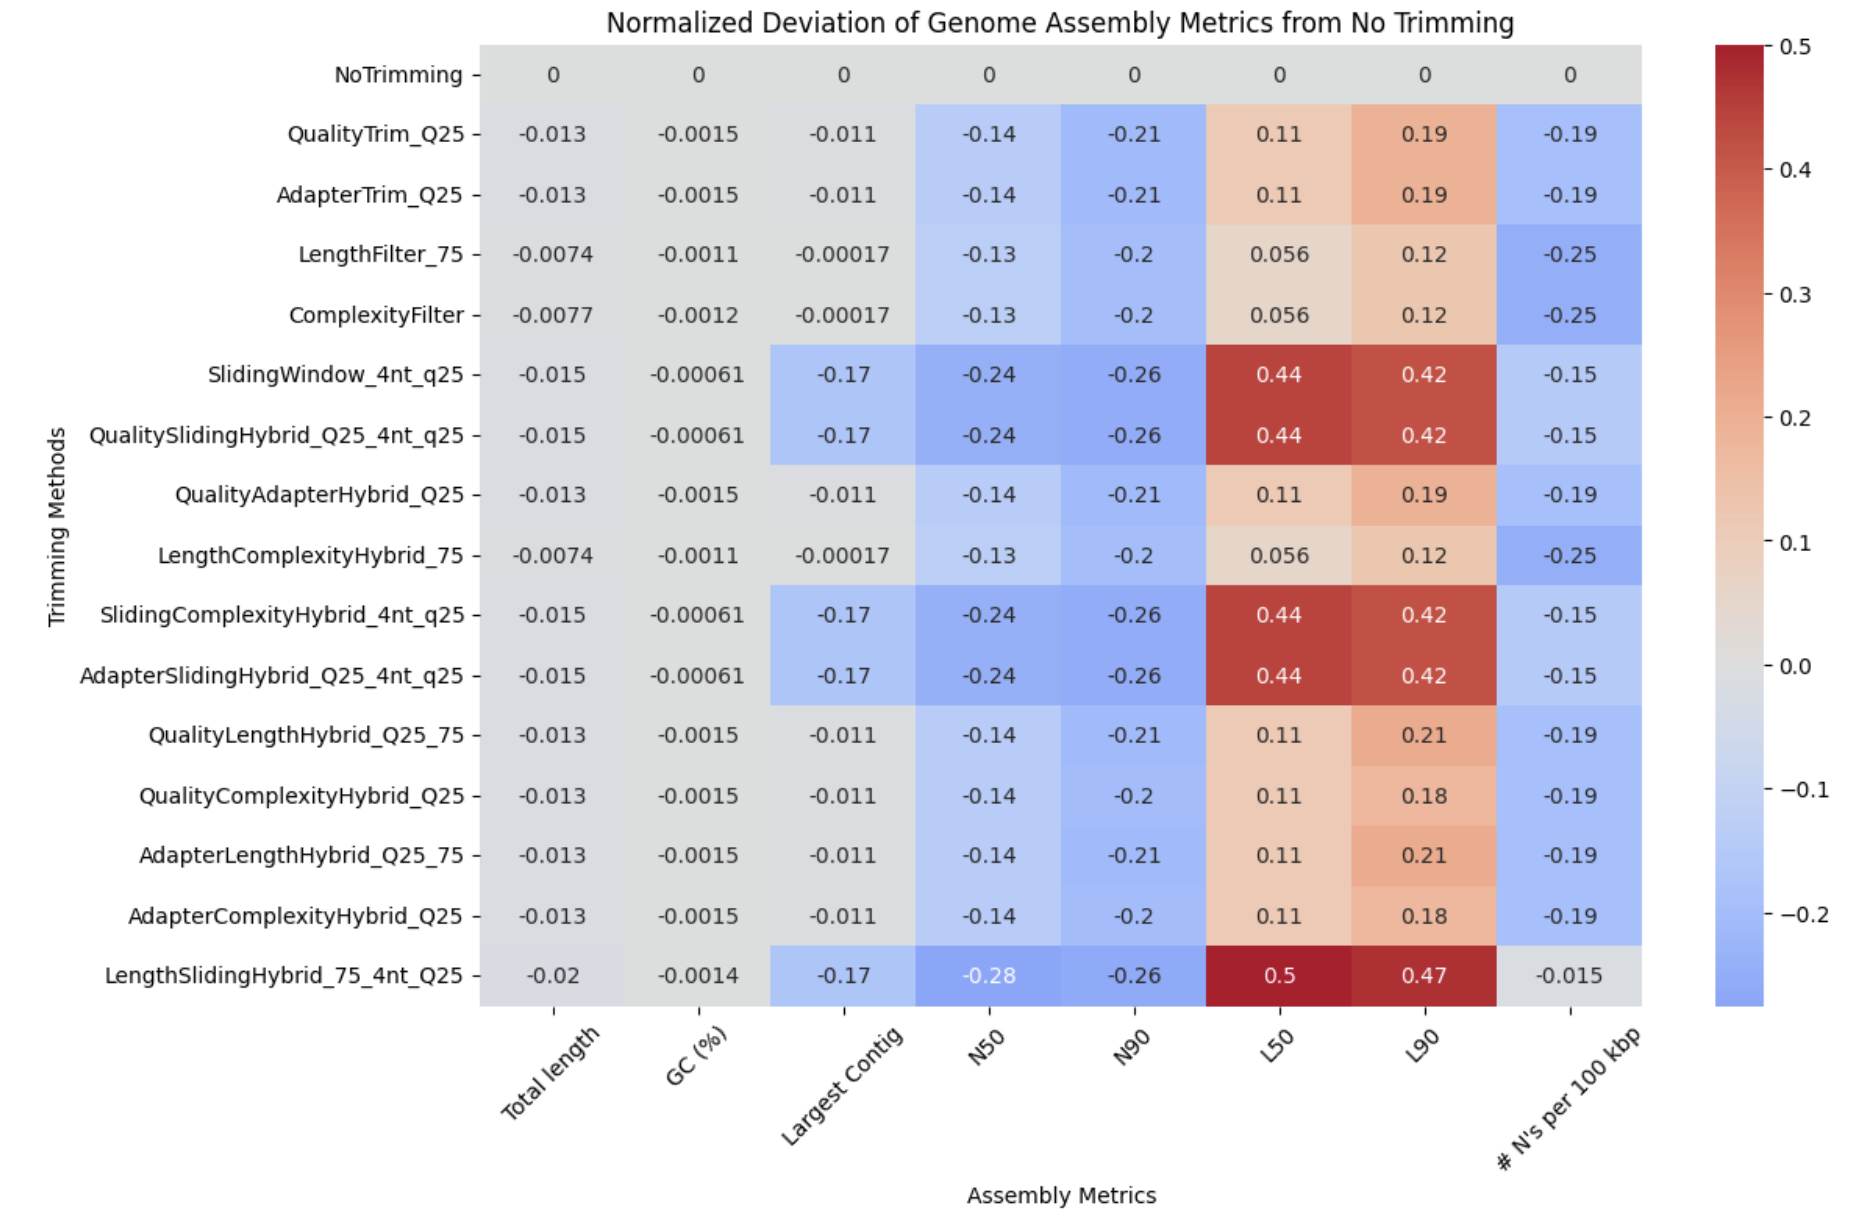
\includegraphics[width=\linewidth]{resources/images/genome_assembly_metrics_heatmap_1.png}
\caption{\textbf{Normalized Deviation of \gls{genome} \gls{metrics} from "No Trimming" — The First \gls{trimming} Strategy}. This \gls{heatmap} illustrates the impact of different \gls{trimming} Methods on various \gls{genome} \gls{metrics}. Darker red indicates a greater positive deviation from \textbf{"No Trimming"}, while darker blue indicates a greater negative deviation. \gls{metrics} include \gls{total length}, \gls{gc}, \gls{largest contigs}, \gls{n50}, \gls{n90}, \gls{l50}, \gls{l90}, and \gls{n's per 100 kbp}.}
\label{fig:genome_assembly_metrics_heatmap_1}
\end{figure}

\textit{The subsequent step involved normalizing the data: this process is described in the \autoref{sec:data_normalization}, where the use of the \autoref{lst:data_norm} is explained in detail.}


A new DataFrame "norm\_deviations" was then generated from a rows\_list consisting of dictionaries, with each dictionary representing a row populated with normalized values.

\textit{The \autoref{fig:genome_assembly_metrics_heatmap_1} was created as a result of execution  the \autoref{lst:heatmap} described in the \autoref{sec:visualization_heatmap}.}



Using the seaborn.heatmap() function, an attempt was made to create a \gls{heatmap} (\autoref{fig:genome_assembly_metrics_heatmap_1}) that eloquently depicts the \gls{deviation} of \gls{genome} \gls{metrics} with respect to the \textbf{"No Trimming"} method. In the spatial configuration of the \gls{heatmap}, rows symbolized the different \gls{trimming} Parameters and columns symbolized the different \gls{genome} \gls{metrics}.

The color of the \gls{heatmap} cells was carefully calibrated to represent the magnitude of \gls{deviation} variances, with the midpoint anchored to zero. Thus, the gradation from red to blue hues indicated the transition from positive to negative \gls{deviation}, respectively. This color scheme was chosen to facilitate intuitive perception of data outliers by providing a sharp visual contrast that highlights the comparative effectiveness of different \gls{trimming} Methods.





\subsection{Evaluating the Trimming Method's Initial Impact} 


\begin{enumerate}
  \item \gls{total length} and \gls{gc} content are largely unaffected (\autoref{fig:genome_assembly_metrics_heatmap_1}) by \gls{trimming} Methods, indicating data consistency and high \gls{sequencing} Quality.
  \item \textbf{Sliding Window \gls{trimming}}, in all its combinations, leads to a significant decrease in \gls{n50} and \gls{n90}, suggesting an over-aggressive approach that negatively impacts \gls{assembly}.
  \item An increase in \gls{l50} and \gls{l90} across several methods indicates more fragmentation and reduced \gls{assembly} Continuity.
  \item \textbf{LengthFilter\_75} and \textbf{ComplexityFilter} methods are noted for their ability to reduce indefinite nucleotides, improving \gls{assembly} Auality and Continuity.
  \item A compromise exists between error reduction and \gls{assembly} Continuity, which needs to be balanced for optimal \gls{assembly} Outcomes.
  \item Further analysis is suggested to assess the compromise between Uncertainty and Continuity \gls{metrics}, possibly through additional hierarchical plotting of the \gls{trimming} Methods.
\end{enumerate}

\subsection{Visual Assessment of Trimming Efficiency} 

\begin{figure}[H]
\centering
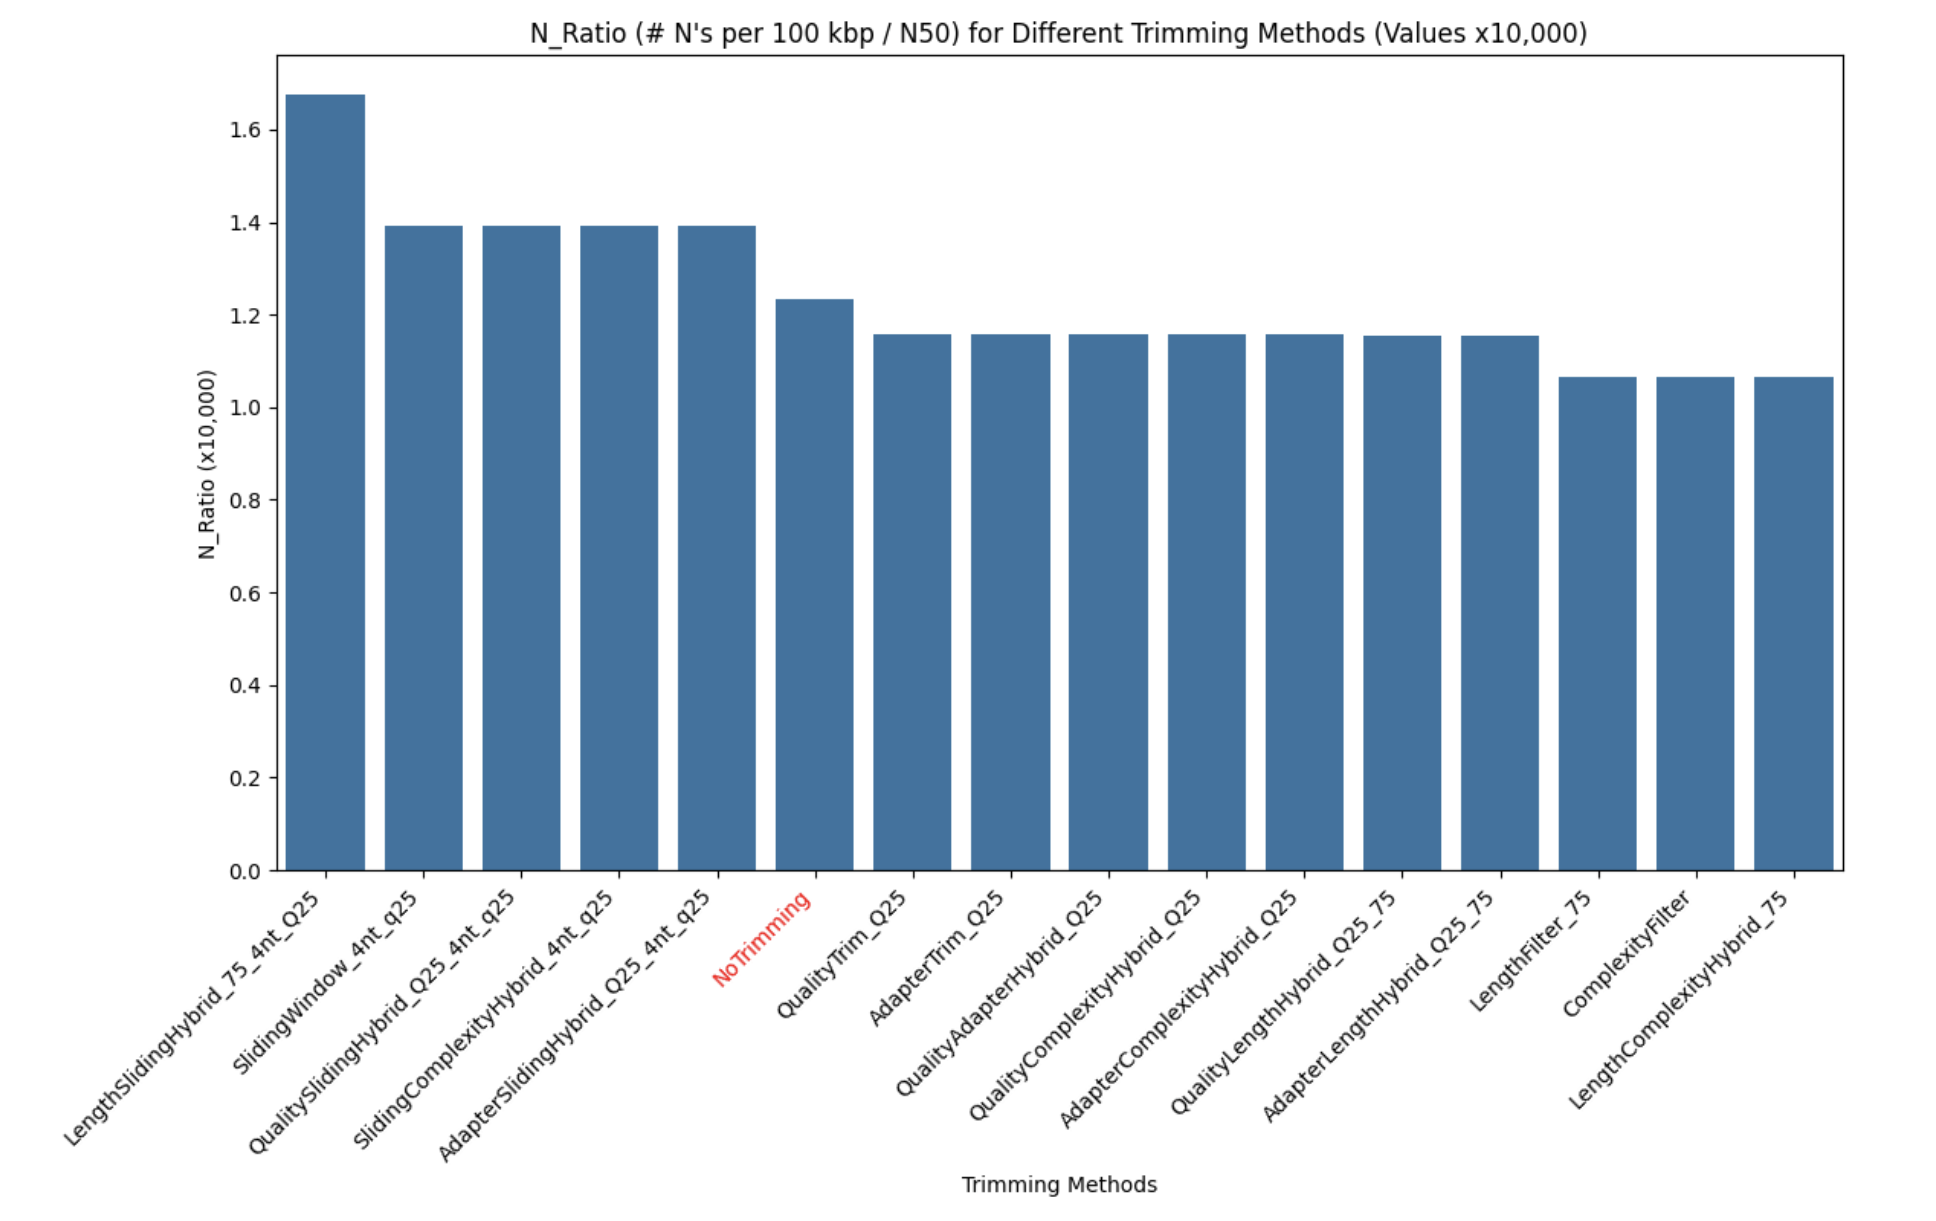
\includegraphics[width=\linewidth]{resources/images/n_ratio_1.png}
\caption{\textbf{The First \gls{trimming} Strategy: the \gls{bar} represents the N ratio — the \gls{n's per 100 kbp} to the \gls{n50} metric for different \gls{trimming} Methods}, with values multiplied by 10,000. The \textbf{'No Trimming'} method serves as a reference point. Each bar represents a different \gls{trimming} Method, and the height of the bar indicates the normalized impact of that method on the \gls{assembly} Quality. A higher bar denotes a method that results in a higher \gls{n's per 100 kbp} relative to the \gls{n50}, suggesting a decrease in \gls{assembly} Quality.}
\label{fig:n_ratio_trim_methods_1}
\end{figure}

\textit{The \autoref{fig:n_ratio_trim_methods_1} was obtained by creating the  N\_ratio, its description is in the  \autoref{sec:calculation_n_ratio}, where the \autoref{lst:n_ratio_calc} performs its computation, and the \autoref{sec:visualization_n_ratio} describes the visualisation of the N\_ratio using the \autoref{lst:n_ratio_visual}.}

\subsection{Refining Trimming Parameters Based on Initial Insights} 

\begin{enumerate}
  \item \gls{trimming} Methods generally outperform (\autoref{fig:n_ratio_trim_methods_1}) \textbf{"No Trimming"} by reducing the \gls{n's per 100 kbp} without compromising \gls{assembly} Continuity, except for methods involving the \textbf{Sliding Window}.
  \item \textbf{LengthFilter\_75}, \textbf{ComplexityFilter}, and their \textbf{hybrid} show the most favorable outcomes in balancing continuity with the reduction of uncertain nucleotides.
\end{enumerate}

To further analyze the impact of \gls{trimming} Methods on \gls{assembly} quality, the following steps are proposed:
\begin{enumerate}
  \item Re-run the software pipeline with a variety of parameters for the \textbf{Sliding Window} and \textbf{Length Filter} methods using The Second \gls{trimming} Strategy (\autoref{sec:2nd_trimming_strategy}).
  \item Parameters for the new run should include:
    \begin{itemize}
      \item 16 different settings for \textbf{Sliding Window} (\autoref{tab:comprehensive_trimming_strategies}).
      \item 6 different settings for \textbf{Length Filter} (\autoref{tab:comprehensive_trimming_strategies}).
    \end{itemize}
  \item Compare the outcomes of these runs with the \textbf{"No Trimming"} to determine the optimal parameters for each method.
\end{enumerate}






\section{The Second Trimming Strategy } \label{sec:2nd_trimming_strategy}


\begin{table}[ht!]
\centering
\caption{The Second Trimming Strategy and Its Impact on Assembly Metrics}
\label{tab:trimming_results_second}
\resizebox{\textwidth}{!}{%
\begin{tabular}{|c|l|r|r|r|r|r|r|r|r|}
\hline
\textbf{\#} & \textbf{Trimming Parameters} & \textbf{Total length} & \textbf{GC (\%)} & \textbf{Largest Contig} & \textbf{N50} & \textbf{N90} & \textbf{L50} & \textbf{L90} & \textbf{\# N's per 100 kbp} \\ \hline
0 & NoTrimming & 4404338 & 65.49 & 209132 & 74608 & 21687 & 18 & 57 & 9.20 \\
1 & SlidingWindow\_4nt\_q15 & 4371714 & 65.47 & 209097 & 66370 & 19392 & 19 & 61 & 7.14 \\
2 & SlidingWindow\_4nt\_q20 & 4355072 & 65.47 & 196013 & 66370 & 16891 & 19 & 66 & 6.92 \\
3 & SlidingWindow\_4nt\_q25 & 4338271 & 65.45 & 173819 & 56417 & 16144 & 26 & 81 & 7.86 \\
4 & SlidingWindow\_4nt\_q30 & 4324613 & 65.42 & 156069 & 45172 & 12240 & 31 & 100 & 4.64 \\
5 & SlidingWindow\_7nt\_q15 & 4386621 & 65.47 & 209097 & 70975 & 20667 & 18 & 59 & 11.52 \\
6 & SlidingWindow\_7nt\_q20 & 4371385 & 65.48 & 196013 & 65416 & 16973 & 20 & 65 & 11.75 \\
7 & SlidingWindow\_7nt\_q25 & 4352562 & 65.46 & 196013 & 64262 & 16735 & 22 & 70 & 7.39 \\
8 & SlidingWindow\_7nt\_q30 & 4335609 & 65.44 & 161559 & 53760 & 15315 & 27 & 84 & 10.41 \\
9 & SlidingWindow\_10nt\_q15 & 4389356 & 65.48 & 209097 & 74525 & 20679 & 18 & 57 & 11.51 \\
10 & SlidingWindow\_10nt\_q20 & 4426558 & 65.49 & 141613 & 49888 & 14028 & 29 & 91 & 20.93 \\
11 & SlidingWindow\_10nt\_q25 & 4359481 & 65.47 & 196013 & 65247 & 16891 & 20 & 66 & 7.15 \\
12 & SlidingWindow\_10nt\_q30 & 4337191 & 65.45 & 141533 & 53760 & 16002 & 27 & 83 & 8.33 \\
13 & SlidingWindow\_20nt\_q15 & 4390654 & 65.47 & 209097 & 70975 & 20679 & 18 & 58 & 9.21 \\
14 & SlidingWindow\_20nt\_q20 & 4377137 & 65.47 & 196013 & 66370 & 19418 & 19 & 61 & 6.91 \\
15 & SlidingWindow\_20nt\_q25 & 4369502 & 65.47 & 196013 & 65416 & 17217 & 21 & 66 & 11.75 \\
16 & SlidingWindow\_20nt\_q30 & 4347271 & 65.46 & 161570 & 64262 & 16677 & 23 & 74 & 10.16 \\
17 & LengthFilter\_50 & 4370507 & 65.41 & 209097 & 65136 & 17421 & 19 & 64 & 6.94 \\
18 & LengthFilter\_75 & 4371727 & 65.42 & 209097 & 65136 & 17421 & 19 & 64 & 6.94 \\
19 & LengthFilter\_100 & 4371227 & 65.42 & 209075 & 64713 & 17421 & 20 & 65 & 6.94 \\
20 & LengthFilter\_150 & 4371488 & 65.42 & 205948 & 64262 & 17416 & 20 & 66 & 6.94 \\
21 & LengthFilter\_200 & 4368193 & 65.42 & 205900 & 64262 & 17416 & 20 & 66 & 7.18 \\
22 & LengthFilter\_250 & 4431464 & 65.42 & 146203 & 41434 & 14197 & 34 & 102 & 16.41 \\
\hline
\end{tabular}%
}
\end{table}


\textit{The data in the \autoref{tab:trimming_results_second} results from reports generated by the second run of the pipeline (\autoref{sec:generated_data}), its extraction with the \autoref{lst:extracting_metrics} calling the \autoref{lst:extraction-function}, and sorting by using the \autoref{lst:sorting_extracted_metrics}, described in the  \autoref{sec:data_extraction}.}

\subsection{Normalization of Comparative Data}

\textit{The subsequent step involved normalizing the data: this process is described in the \autoref{sec:data_normalization}, where the use of the \autoref{lst:data_norm} is explained in detail.}

\subsection{Heatmap Visualization of Refined Data}

\textit{The \autoref{fig:genome_assembly_metrics_heatmap_2} was created as a result of execution the \autoref{lst:heatmap} described in the  \autoref{sec:visualization_heatmap}.}

\begin{figure}[H]
\centering
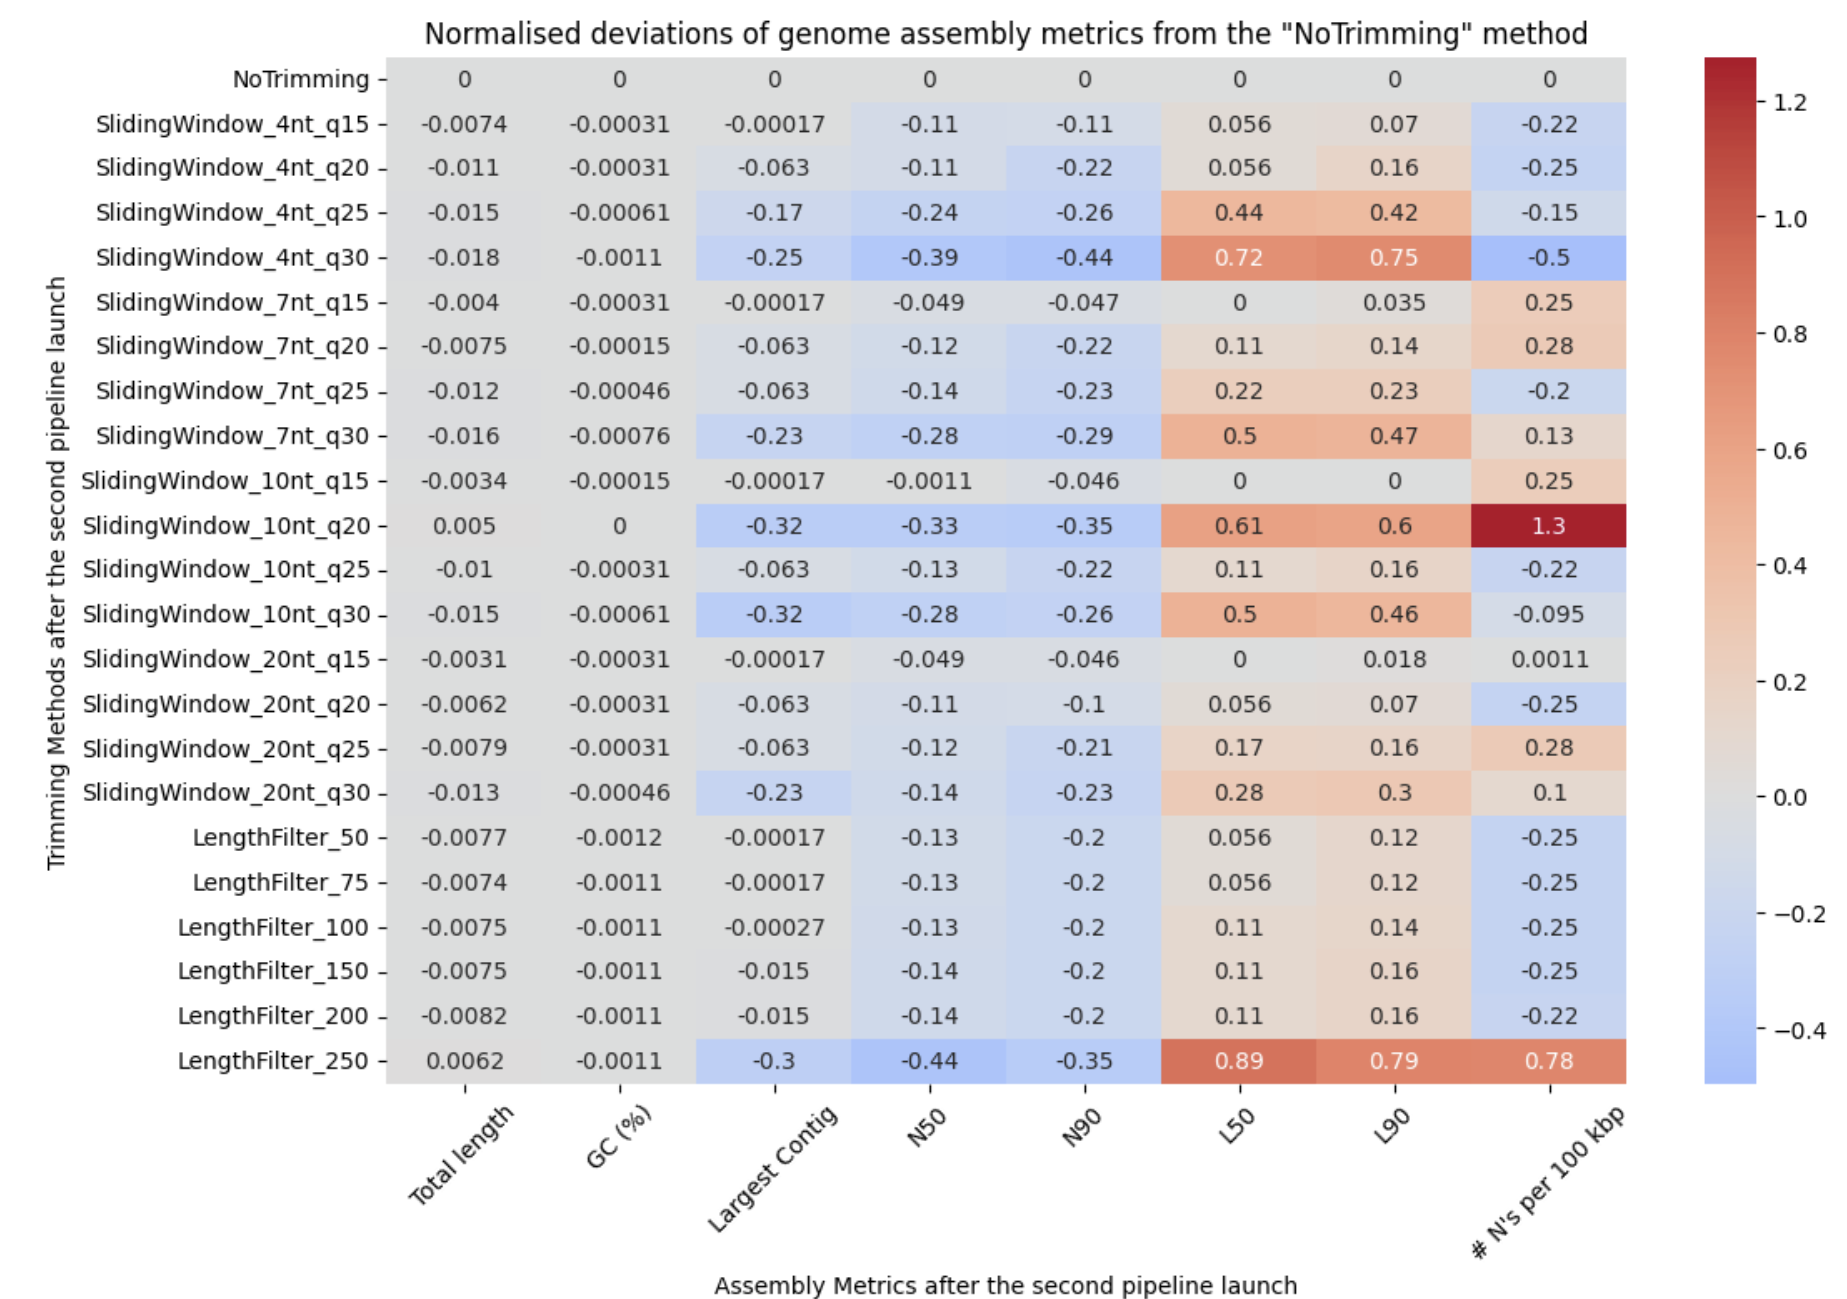
\includegraphics[width=\linewidth]{resources/images/genome_assembly_metrics_heatmap_2.png}
\caption{\textbf{\gls{deviation} of \gls{genome} \gls{metrics} from "No Trimming" — The Second \gls{trimming} Strategy}. This visual representation highlights the impact of different \textbf{Sliding Window} and \textbf{Length Filter} parameters on \gls{metrics} such as \gls{total length}, \gls{gc}, \gls{largest contigs}, \gls{n50}, \gls{n90}, \gls{l50}, \gls{l90}, and \gls{n's per 100 kbp}. Notably, certain parameters show a marked decrease in \gls{n50} and increase in \gls{l50}, \gls{l90}, suggesting a compromise between \gls{trimming} Stringency and \gls{assembly} Continuity.}
\label{fig:genome_assembly_metrics_heatmap_2}
\end{figure}



\subsection{Assessment of Refined Trimming Parameters}

\begin{enumerate}
  \item As the \gls{n's per 100 kbp} decreases (\autoref{fig:genome_assembly_metrics_heatmap_2}), there is a corresponding decrease in \gls{n50} and \gls{n90}, and an increase in \gls{l50} and \gls{l90}, highlighting a consistent pattern across \gls{trimming} Methods.
  \item Some \gls{trimming} Methods, such as \textbf{SlidingWindow\_7nt\_q15}, lead to an increased number of N's without significantly altering other parameters, indicating a poor \gls{trimming} Performance.
  \item Extreme cases, like \textbf{SlidingWindow\_10nt\_q20} and \textbf{LengthFilter\_250}, cause a drastic reduction in \gls{assembly} Quality.
\end{enumerate}

To further understand the impact of \gls{trimming} Methods:
\begin{enumerate}
  \item An additional plot (\autoref{fig:n_ratio_after_second_pipeline}) will be created to rank the \gls{trimming} Methods by the ratio of the frequency of N's to the \gls{n50} metric, thereby establishing a hierarchy of method effectiveness.
\end{enumerate}

\subsection{Bar Chart Analysis of N Ratio Improvements} 

\textit{The \autoref{fig:n_ratio_after_second_pipeline} was obtained by creating the N\_ratio, its description is in the  \autoref{sec:calculation_n_ratio}, where the \autoref{lst:n_ratio_calc} performs its computation, and the \autoref{sec:visualization_n_ratio} describes the visualisation of the N\_ratio using the  \autoref{lst:n_ratio_visual}.}

\begin{figure}[h!]
\centering
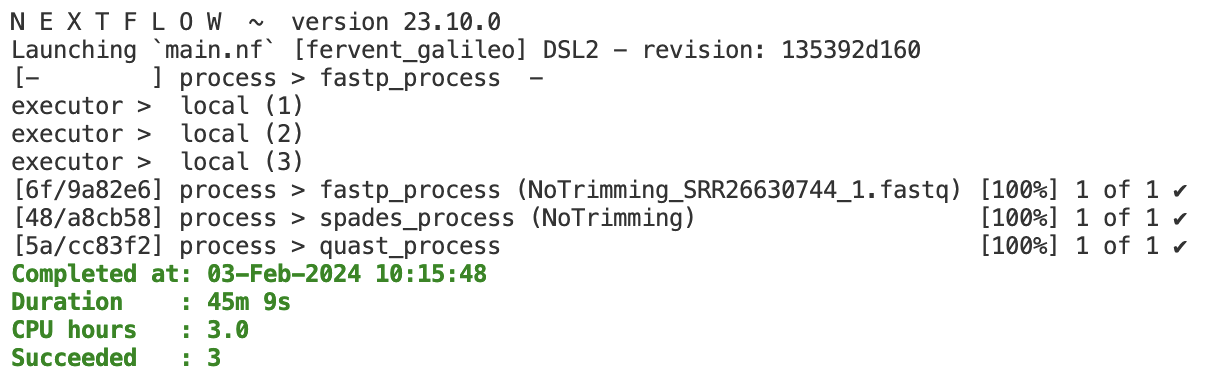
\includegraphics[width=\linewidth]{resources/images/nextflow_output.png}
\caption{\textbf{An example of an output of the Nextflow pipeline execution}, version 23.10.0, showcasing the completion of various bioinformatics processes. The workflow includes processes such as 'fastp\_process', 'spades\_process', and 'quast\_process' with inputs like 'NoTrimming\_SRR26630744\_1.fastq'. The execution was completed on 03-Feb-2024 at 10:15:48, taking a total duration of 45 minutes and 9 seconds, consuming 3.0 CPU hours, and successfully completing three processes for the single "NoTrimming" Method.}
\label{fig:nextflow_output}
\end{figure}

\begin{figure}[H]
\centering
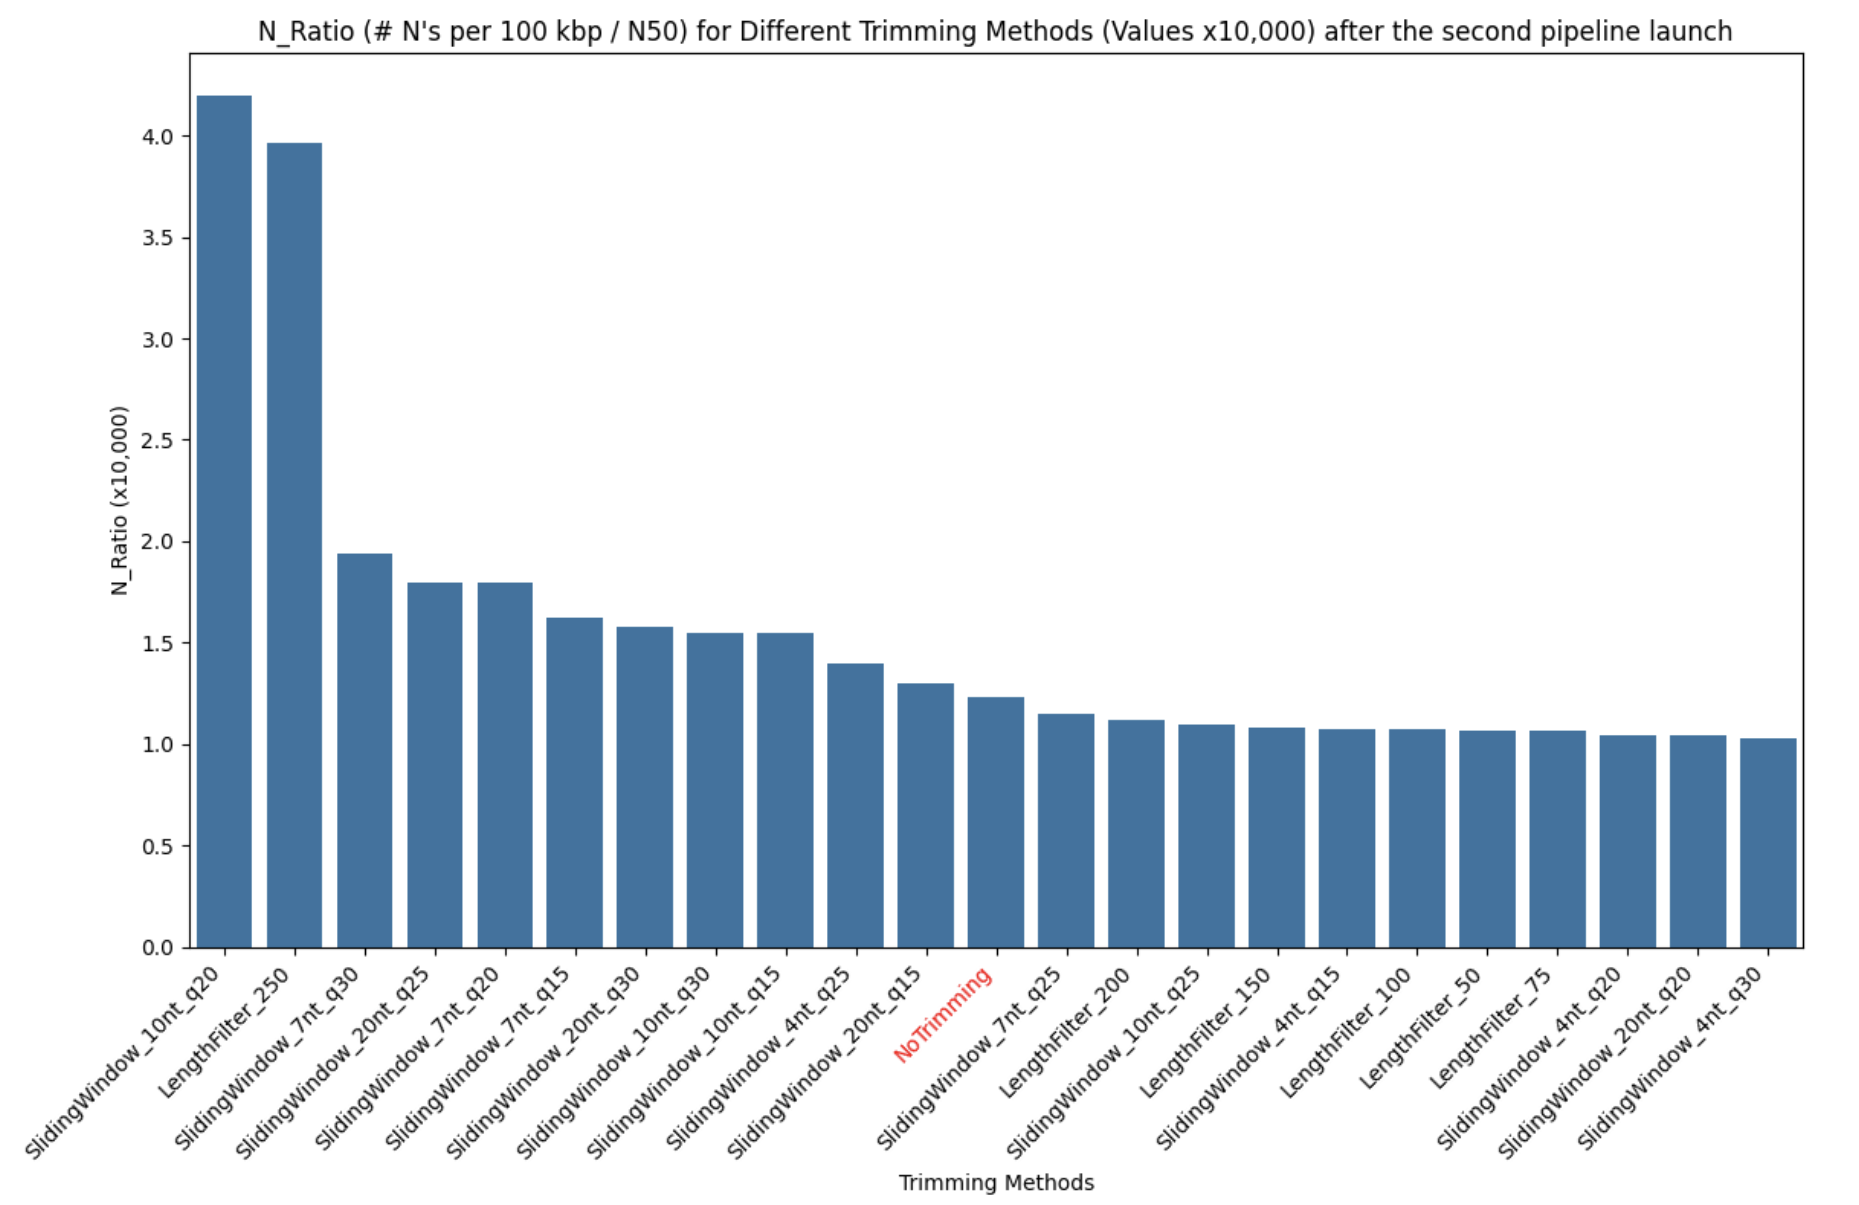
\includegraphics[width=\linewidth]{resources/images/n_ratio_2.png}
\caption{\textbf{The Second \gls{trimming} Strategy: the \gls{bar} showing the N\_Ratio, which is the \gls{n's per 100 kbp} divided by the \gls{n50} metric, for different \gls{trimming} Methods} following the second pipeline run. The values are multiplied by 10,000 to facilitate comparison. The \textbf{'No Trimming'} method serves as a benchmark. A higher bar denotes a method that results in a higher \gls{n's per 100 kbp} relative to the \gls{n50}, suggesting a decrease in \gls{assembly} Quality.}
\label{fig:n_ratio_after_second_pipeline}
\end{figure}



\subsection{Critical Analysis of Parameter Refinement}

\begin{enumerate}
  \item Certain parameters (\autoref{fig:n_ratio_after_second_pipeline}) of the \textbf{Sliding Window} method, previously considered suboptimal, have shown improved \gls{assembly} Quality upon re-evaluation, even outperforming the previously favored \textbf{LengthFilter\_75} in some instances.
  \item Conversely, some parameters of the initially superior \textbf{Length Filter} method, such as \textbf{LengthFilter\_250}, may not be advantageous, indicating the significance of parameter selection within each method.
\end{enumerate}

Further Insights and Steps:

\begin{enumerate}
  \item The importance of the \gls{trimming} Method's parameters has been experimentally validated, influencing the quality of \gls{assembly}.
  \item The iterative use of the pipeline has refined our understanding of which \gls{trimming} Methods and parameters yield the best \gls{assembly} Quality.
  \item A new visualization approach is proposed using \gls{scatter} (\autoref{fig:length_filter_variation}, \autoref{fig:3d_scatter_sliding_window}) to analyze the variance in \gls{assembly} Quality across different parameters within the \textbf{Sliding Window} and \textbf{Length Filter} methods.
  \item Specifically for \textbf{Length Filter}, the 2D \gls{scatter} (\autoref{fig:length_filter_variation}) will be created to illustrate the relationship between its parameters and the metrics \gls{n50} and the \gls{n's per 100 kbp}.
\end{enumerate}



\subsection{Visualizing Optimal Trimming Outcomes}



\begin{figure}[H]
\centering
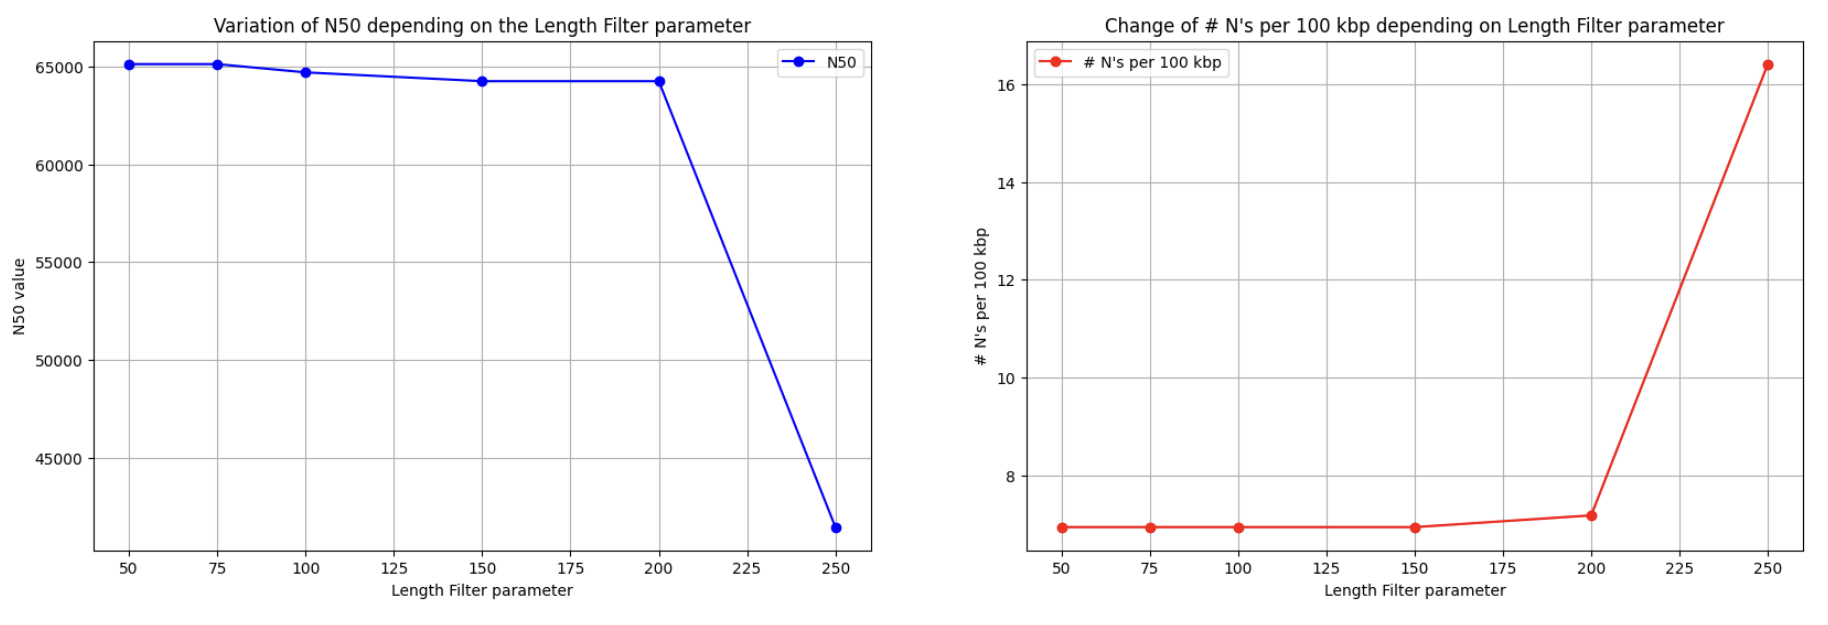
\includegraphics[width=\linewidth]{resources/images/length_filter_variation.png}
\caption{\textbf{The dual \gls{scatter} illustrate the variation of the \gls{n50} metric (left) and the change in the \gls{n's per 100 kbp} (right) as a function of the Length Filter parameter}. The \gls{n50} value remains relatively stable across a range of parameters but sharply decreases after a certain threshold. Conversely, the \gls{n's per 100 kbp} stays consistent before dramatically increasing, indicating a critical parameter value beyond which the \textbf{Length Filter} negatively impacts the \gls{assembly}.}
\label{fig:length_filter_variation}
\end{figure}

\textit{The \autoref{fig:length_filter_variation} was created by using the \autoref{lst:scatter_plot} described in the  \autoref{sec:length_filter_trimming} and in the  \autoref{sec:length_filter_trimming_visualisation}. And the \autoref{fig:3d_scatter_sliding_window} was created by using the \autoref{lst:3d_scatter_plot} described in the  \autoref{sec:sliding_window_trimming} and in the \autoref{sec:sliding_window_trimming_visualisation}. The \autoref{fig:3d_scatter_sliding_window} depicts just a screenshot of the visual program MetricsExtractor, which interactively allows researches to find the best of the best metrics (\autoref{sec:sliding_window_trimming_visualisation}).}


\begin{SCfigure}
  \centering
  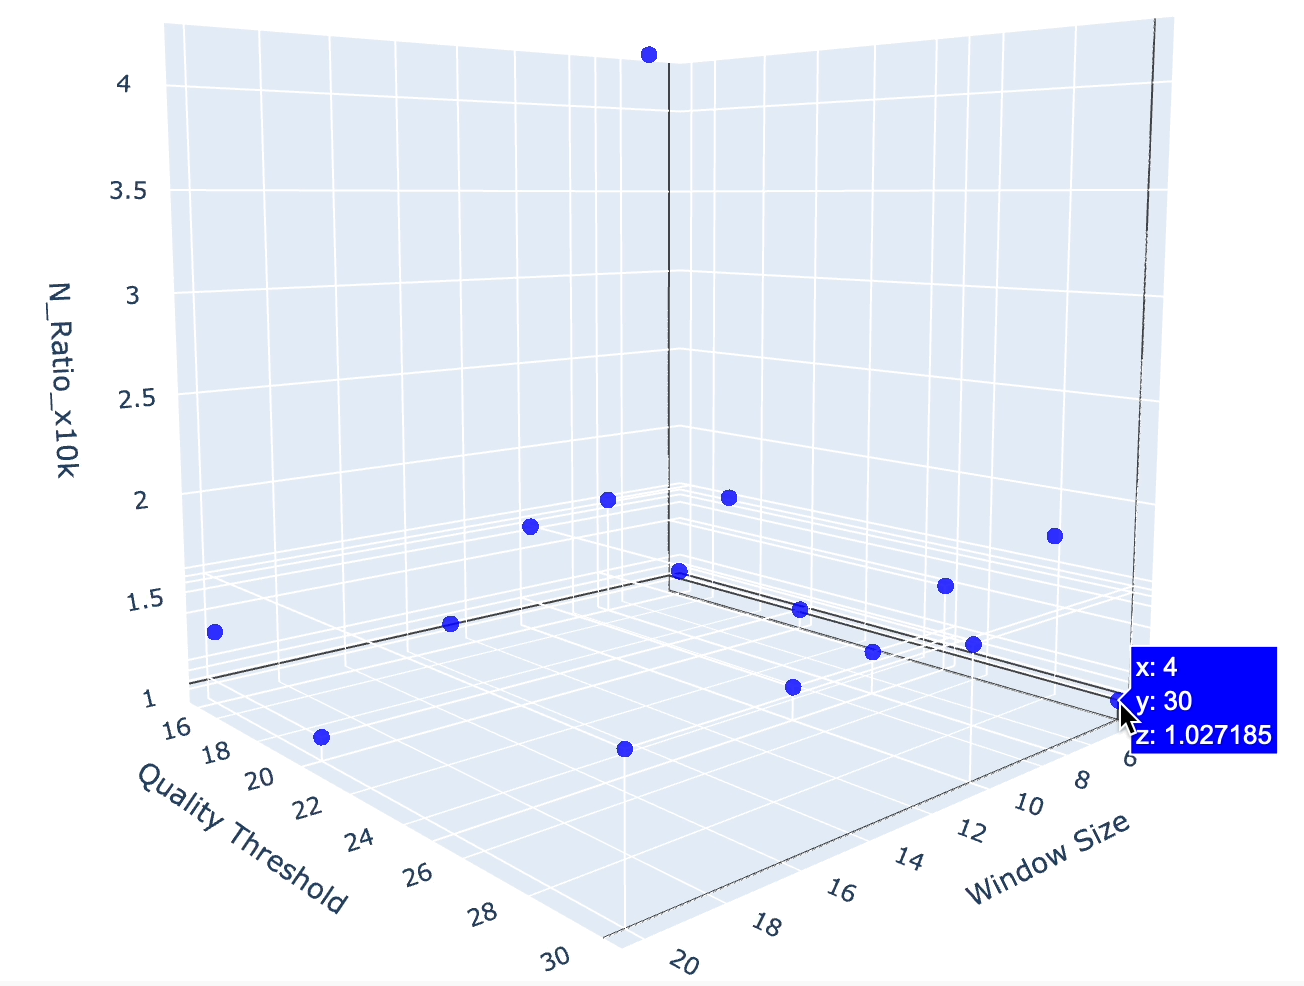
\includegraphics[width=0.48\textwidth]{resources/images/3d_scatter_sliding_window.png}
  \caption{\textbf{The 3D \gls{scatter} representing the N\_Ratio\_x10k of the Sliding Window \gls{trimming} Method as a function of its parameters}, specifically window size and quality threshold. The plot points are distributed across the three-dimensional space defined by these two parameters and the resulting N\_Ratio\_x10k, highlighting the complex relationship between \gls{trimming} Method parameters and the impact on \gls{assembly} Quality.}
  \label{fig:3d_scatter_sliding_window}
\end{SCfigure}



\subsection{Final Evaluation of Trimming Strategy Efficacy}

\begin{enumerate}
  \item The \gls{scatter}s (\autoref{fig:length_filter_variation}, \autoref{fig:3d_scatter_sliding_window}) reveal an inverse relationship between the \gls{n50} metric and the \gls{n's per 100 kbp}, illustrating the impact of the \textbf{Length Filter} parameter on \gls{assembly} Quality.
  \item Parameters in the range of 50 to 75 for the Length Filter method are indicated to potentially enhance \gls{assembly} Quality.
  \item A proposal is made to re-run the pipeline with \textbf{Length Filter} parameters around 50-75 to possibly improve \gls{assembly} Quality further.
  \item For the \textbf{Sliding Window} method, the 3D \gls{scatter} (\autoref{fig:3d_scatter_sliding_window}) is suggested to analyze the N\_Ratio\_x10k against its varying parameters, necessitating data filtering to select for \textbf{Sliding Window} parameters exclusively.
  \item The interactive 3D \gls{scatter} allows us to examine each data point alongside its corresponding X (window size), Y (mean quality), and Z (N\_Ratio\_x10k) values, illustrating the \gls{trimming} Method's parameter effects on \gls{assembly} Quality.
  \item The point with the lowest Z value on the plot indicates the optimal parameters for the \textbf{Sliding Window} method that achieve the best balance between the \gls{n's per 100 kbp} and \gls{n50}, suggesting a superior \gls{assembly} Quality.
  \item Initiating a third pipeline run with parameters near this optimal point may potentially refine the quality of \gls{genome} \gls{trimming} even further.
\end{enumerate}





\section{The Third Trimming Strategy }  \label{sec:3rd_trimming_stratrgy}


\begin{table}[ht!]
\centering
\caption{The Third Trimming Strategy and Its Impact on Assembly Metrics}
\label{tab:trimming_results_third}
\resizebox{\textwidth}{!}{%
\begin{tabular}{|c|l|r|r|r|r|r|r|r|r|}
\hline
\textbf{\#} & \textbf{Trimming Parameters} & \textbf{Total length} & \textbf{GC (\%)} & \textbf{Largest Contig} & \textbf{N50} & \textbf{N90} & \textbf{L50} & \textbf{L90} & \textbf{\# N's per 100 kbp} \\ \hline
0 & SlidingWindow\_3nt\_q30 & 4302594 & 65.40 & 139540 & 38864 & 10691 & 34 & 111 & 1.86 \\
1 & SlidingWindow\_4nt\_q30 & 4310805 & 65.42 & 156069 & 45172 & 12240 & 31 & 100 & 4.64 \\
2 & SlidingWindow\_4nt\_q29 & 4314963 & 65.43 & 161279 & 49758 & 12487 & 29 & 94 & 6.49 \\
3 & SlidingWindow\_5nt\_q30 & 4315324 & 65.43 & 161302 & 45552 & 12261 & 31 & 98 & 6.49 \\
4 & LengthFilter\_30 & 4321024 & 65.41 & 209097 & 65136 & 17421 & 19 & 64 & 6.94 \\
5 & LengthFilter\_35 & 4321024 & 65.41 & 209097 & 65136 & 17421 & 19 & 64 & 6.94 \\
6 & LengthFilter\_40 & 4321012 & 65.41 & 209097 & 65136 & 17421 & 19 & 64 & 6.94 \\
7 & LengthFilter\_45 & 4321017 & 65.41 & 209097 & 65136 & 17421 & 19 & 64 & 6.94 \\
8 & LengthFilter\_50 & 4321006 & 65.41 & 209097 & 65136 & 17421 & 19 & 64 & 6.94 \\
9 & LengthFilter\_55 & 4321006 & 65.41 & 209097 & 65136 & 17421 & 19 & 64 & 6.94 \\
\hline
\end{tabular}%
}
\end{table}

\textit{The data in the \autoref{tab:trimming_results_third} results from reports generated by the third run of the pipeline (\autoref{sec:generated_data}), its extraction with the \autoref{lst:extracting_metrics} calling the \autoref{lst:extraction-function}, and sorting by using the \autoref{lst:sorting_extracted_metrics}, described in the  \autoref{sec:data_extraction}.}

\textit{The \autoref{fig:length_filter_variation_2} was created by using the \autoref{lst:scatter_plot} described in the  \autoref{sec:length_filter_trimming} and in the  \autoref{sec:length_filter_trimming_visualisation}. And the \autoref{fig:n_ratio_3} was obtained by creating the N\_ratio, its description is in the  \autoref{sec:calculation_n_ratio}, where the \autoref{lst:n_ratio_calc} performs its computation, and the \autoref{sec:visualization_n_ratio} describes the visualisation of the N\_ratio using the  \autoref{lst:n_ratio_visual}.}



\subsection{Comparative Overview of Genome Assembly Metrics}

\begin{figure}[H]
    \centering
    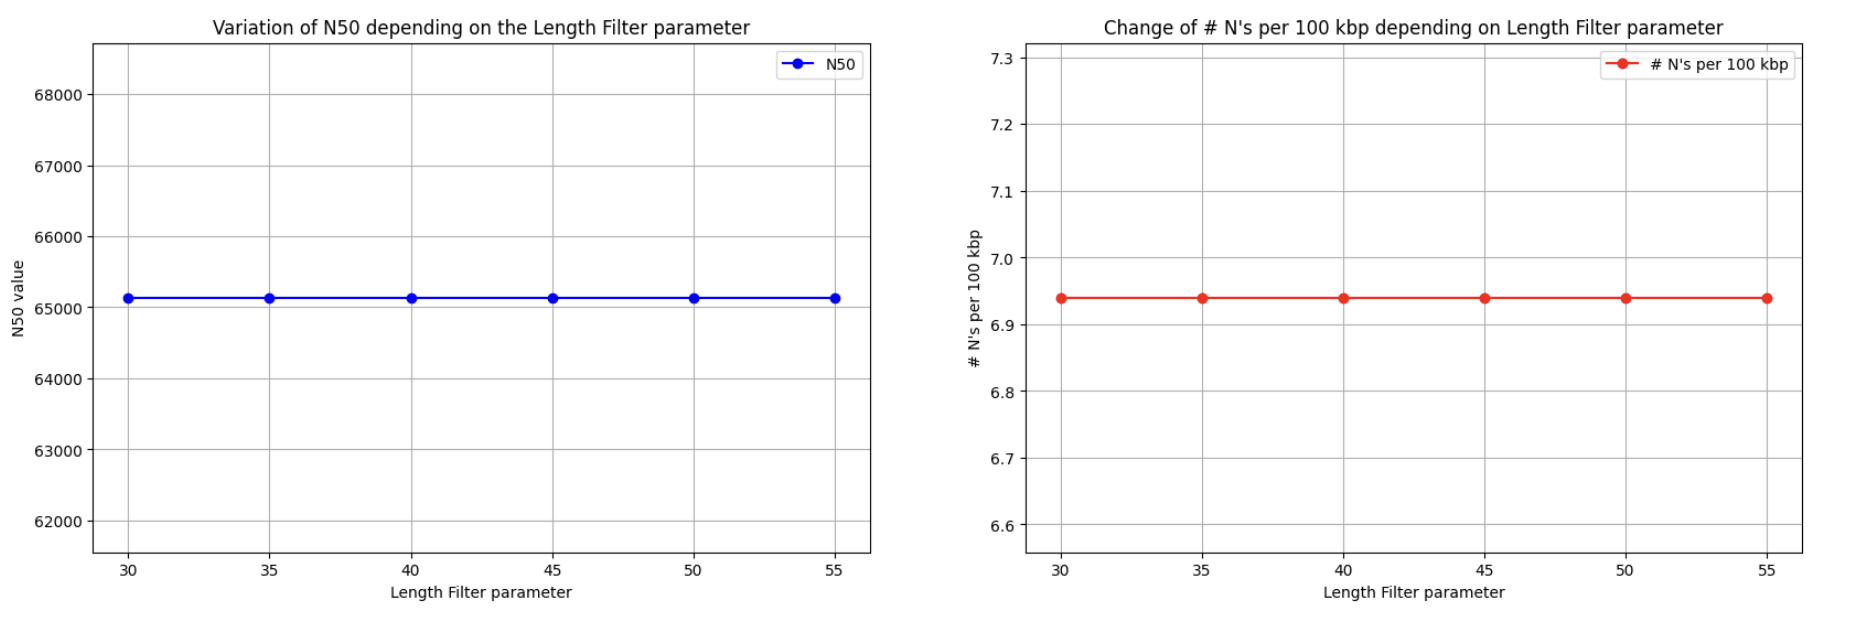
\includegraphics[width=0.7\linewidth]{resources/images/length_filter_variation_2.png}
    \caption{\textbf{Two \gls{scatter}s depicting the variation of the \gls{n50} metric and the change in the \gls{n's per 100 kbp} as functions of the Length Filter parameter.} The left plot shows \gls{n50} values remaining stable across different parameters, while the right plot illustrates a consistent \gls{n's per 100 kbp}, independent of the \textbf{Length Filter} parameter changes. These trends suggest that within the examined parameter range, the \textbf{Length Filter} has a negligible effect on both the continuity and the gap size of the \gls{assembly}.}
    \label{fig:length_filter_variation_2}
    
    \vspace{1cm}
    
    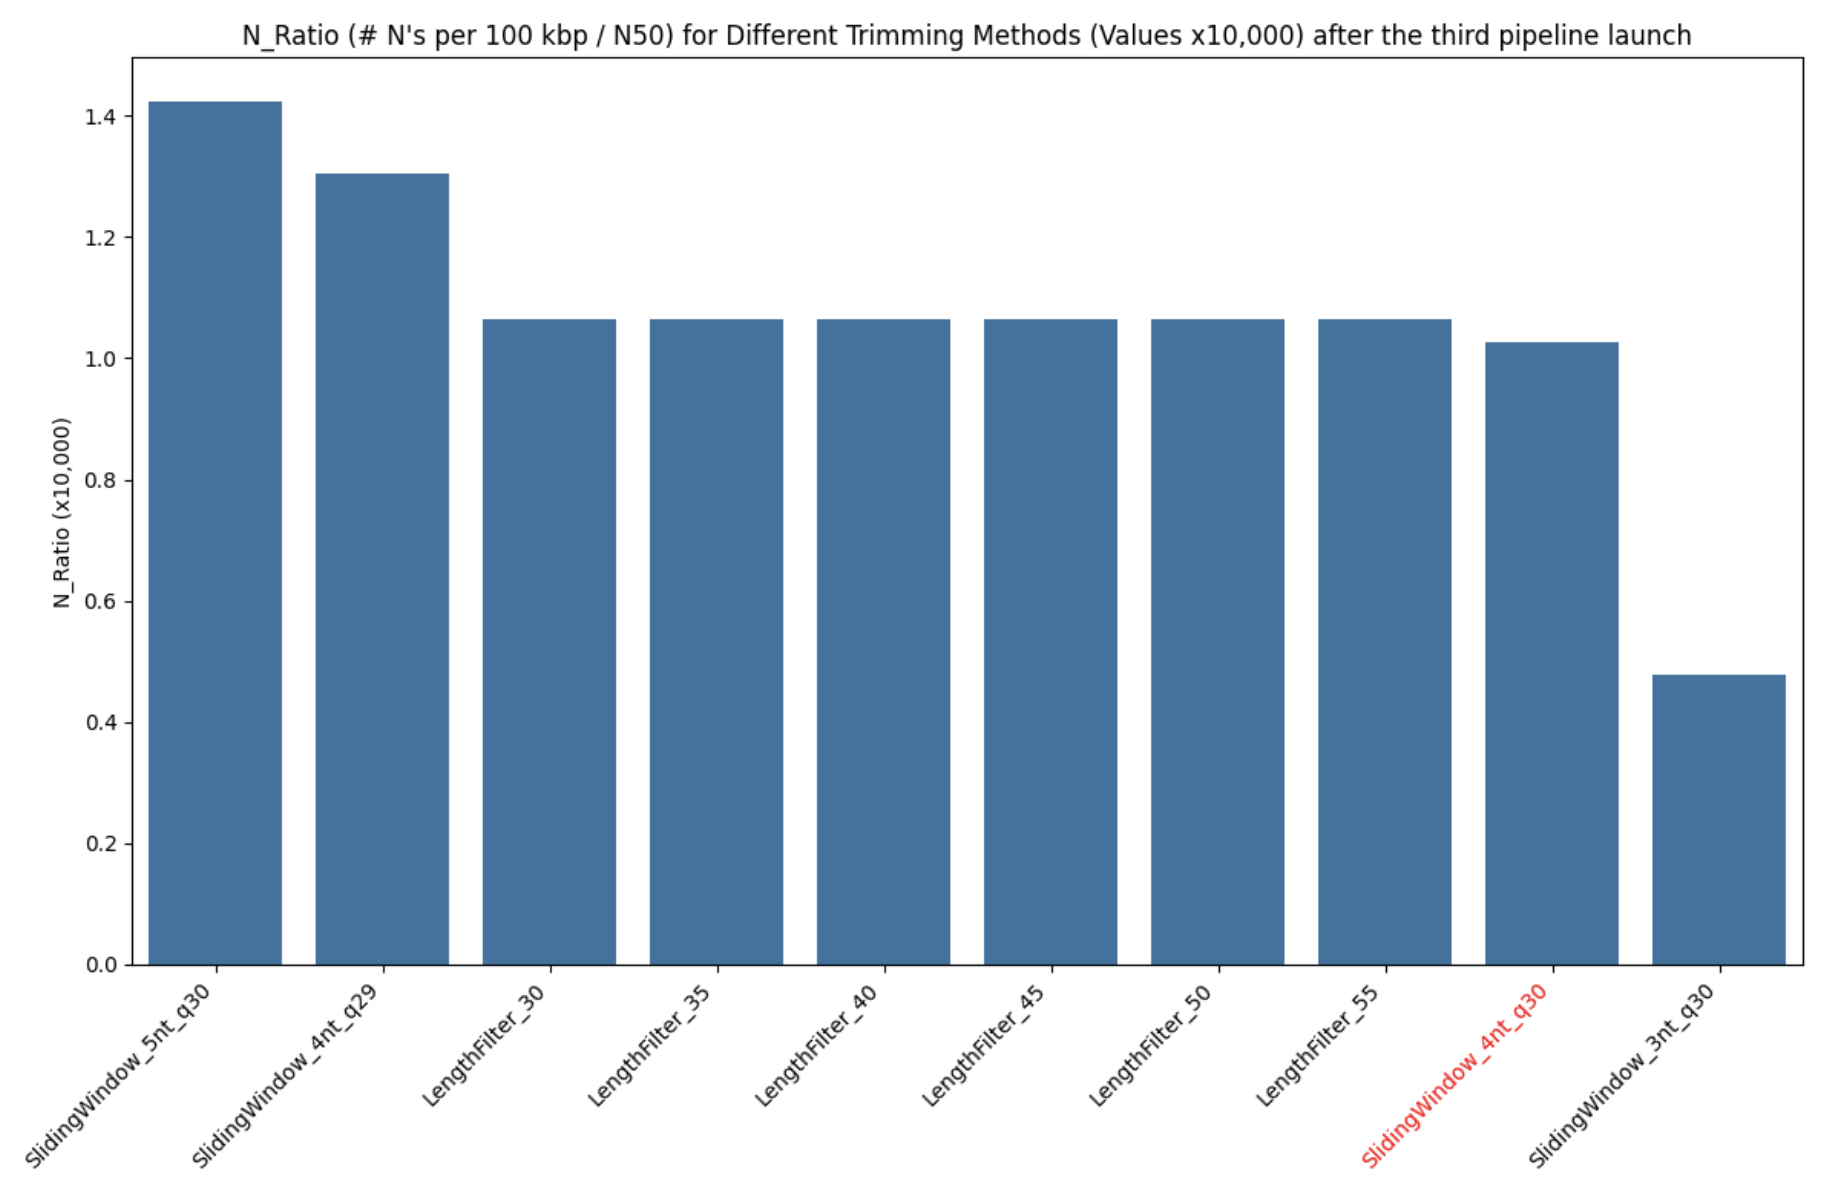
\includegraphics[width=0.7\linewidth]{resources/images/n_ratio_3.png}
    \caption{\textbf{\gls{bar}s showing the N\_Ratio (\gls{n's per 100 kbp} / \gls{n50}) for different \gls{trimming} Methods after the third pipeline run}, multiplied by 10,000. The bars represent various methods, including \textbf{Sliding Window} and \textbf{Length Filter}, with their respective parameter values. The significant decrease in the N\_Ratio for certain parameters indicates a more favorable outcome in \gls{assembly} Quality.}
    \label{fig:n_ratio_3}
\end{figure}



\subsection{Conclusive Insights on Trimming Efficacy}

\begin{enumerate}
    \item The analysis of the graph (\autoref{fig:length_filter_variation_2}) indicates that modifying the \gls{trimming} Method parameters to values near their previously identified optimum does not yield improvement. Consequently, the initial hypothesis was not corroborated by the results.
    \item \autoref{fig:n_ratio_3}: our hypothesis was confirmed, leading to the discovery of an improved data \gls{trimming} method using the \textbf{SlidingWindow\_3nt\_q30} parameters.
\end{enumerate}


\section{A Comparative Analysis}

\begin{figure}[!ht]
    \centering
    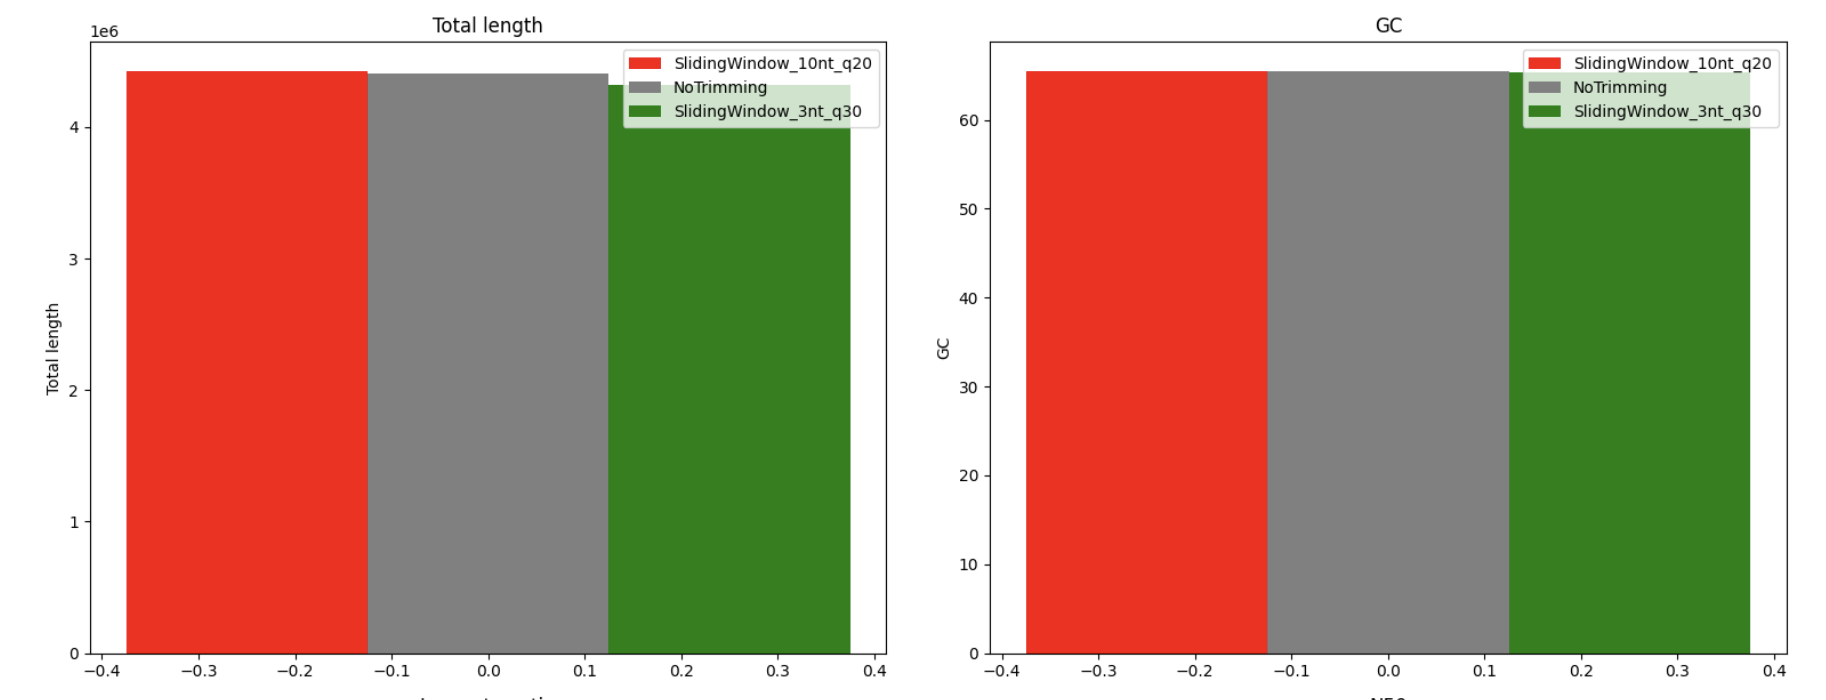
\includegraphics[width=0.8\textwidth]{resources/images/total_length_gc.png}
    \caption{\textbf{\gls{total length} and \gls{gc}} - worst/best}
    \label{fig:total_length_gc}
\end{figure}

\begin{figure}[!ht]
    \centering
    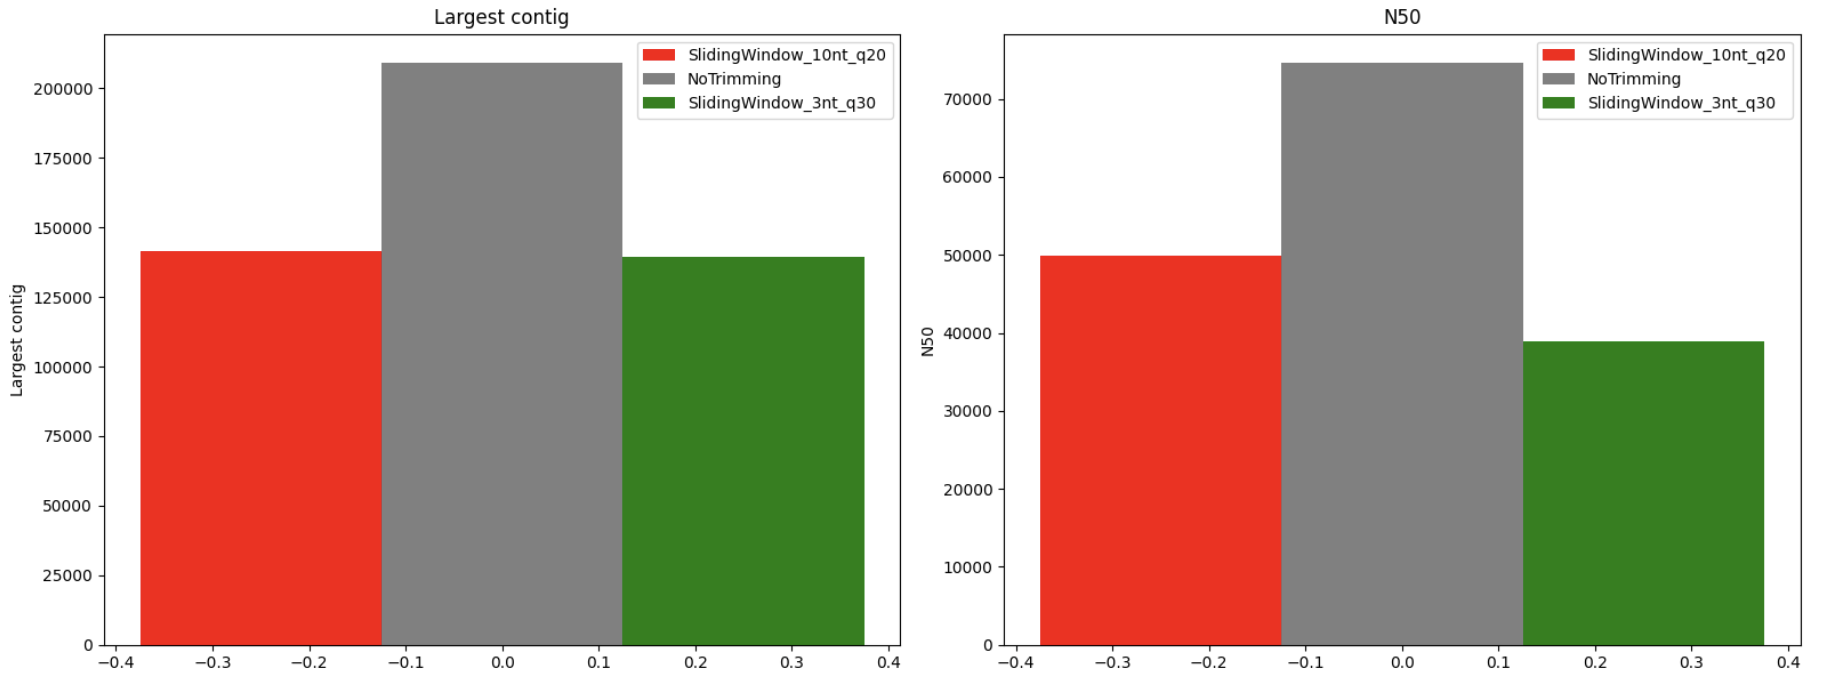
\includegraphics[width=0.8\textwidth]{resources/images/largest_contig_n50.png}
    \caption{\textbf{\gls{largest contigs} and \gls{n50}} - worst/best}
    \label{fig:largest_contig_n50}
\end{figure}

\begin{figure}[!ht]
    \centering
    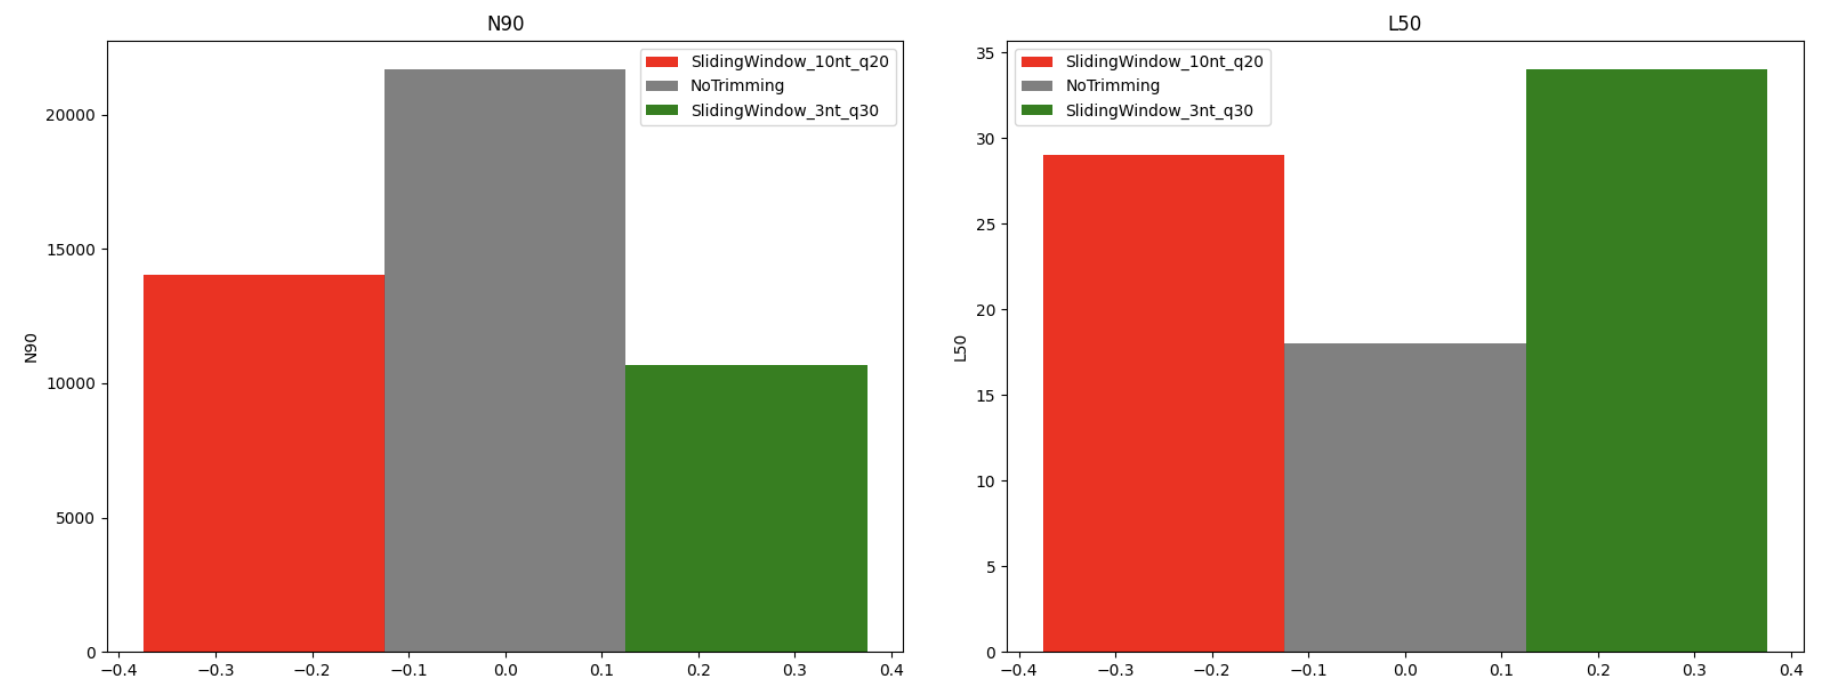
\includegraphics[width=0.8\textwidth]{resources/images/n90_l50.png}
    \caption{\textbf{\gls{n90} and \gls{l50}} - worst/best}
    \label{fig:n90_l50}
\end{figure}

\begin{figure}[!ht]
    \centering
    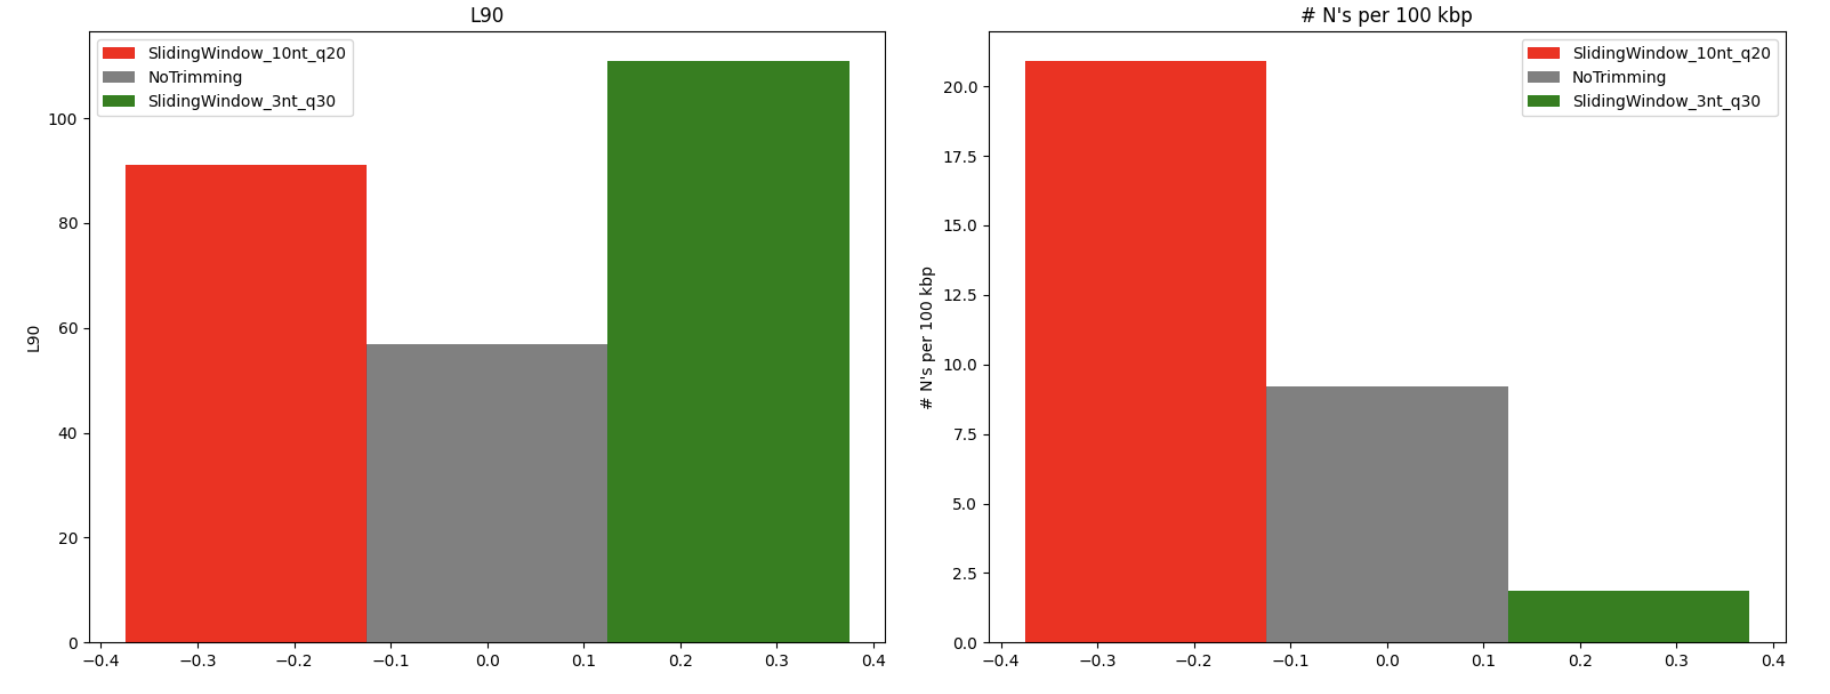
\includegraphics[width=0.8\textwidth]{resources/images/l90_ns_per_100kbp.png}
    \caption{\textbf{\gls{l90} and \gls{n's per 100 kbp}} - worst/best}
    \label{fig:l90_ns_per_100kbp}
\end{figure}


\begin{enumerate}
    \item{Comparative \gls{bar}s of \gls{assembly} Metrics for different \gls{trimming} Methods. Demonstrative comparison of the effects of three \gls{trimming} Methods on different metrics assessing the quality of \gls{assembly}. The best \gls{trimming} Method found (\textbf{SlidingWindow\_3nt\_q30}) demonstrates the advantage of using the pipeline.}
    \item Through iterative execution of the pipeline and intermediate data processing, we identified the most and least effective data \gls{trimming} Methods (\autoref{fig:l90_ns_per_100kbp}), depicted in green and red respectively, against the \textbf{"No Trimming"} (gray) scenario.
    \item The optimal \gls{trimming}  Method, \textbf{SlidingWindow\_3nt\_q30}, demonstrated the lowest N\_Ratio value among all tested, indicating the highest efficiency in reducing the \gls{n's per 100 kbp}  relative to \gls{n50}.
    \item The improvement factor for the best \gls{trimming} Method over the no-trimming scenario was \textbf{4.95} in terms of \gls{n's per 100 kbp} , showcasing significant enhancement in data quality. The \gls{n50}  indicator decreased by \textbf{1.9} times compared to when \gls{trimming}  was not used.
\end{enumerate} \clearpage
\chapter{Discussion}

\textbf{Study Overview and Reproducibility.} This study embarked upon a comprehensive exploration of various trimming strategies applied to sequenced data, with the aim of discerning their impact on the quality of genomic assembly. To ensure the reproducibility of our results, meticulous documentation of every procedural step, utilized parameters, and data processing conditions was maintained. This effort culminates in the provision of all data, alongside the LaTeX documentation of this work, which is made available in Section \ref{sec:generated_data} of the mentioned repository, facilitating future research endeavors.

\textbf{Results Interpretation and Novel Metric Introduction.} In the results section (Section \ref{sec:results}), we delved into a detailed interpretation of the findings, shedding light on the merits and limitations inherent to each trimming approach. A pivotal aspect of this study is the introduction of a novel metric, termed the N\_value, specifically devised to evaluate the efficacy of different trimming methods. This investigation led to the proposition of three iterative trimming strategies, detailed in sections \ref{sec:1st_trimming_stratrgy}, \ref{sec:2nd_trimming_strategy}, and \ref{sec:3rd_trimming_stratrgy}, through which we identified the most efficacious approach.

\textbf{Significance of the Software Pipeline.} The empirical evidence gathered through this research underscores the significance of the software pipeline developed, affirming its utility as an effective tool in the scientific research arsenal. We encourage fellow researchers in the field to engage with the techniques delineated herein and embark on their quest to refine data trimming strategies, aiming to enhance the stability and reliability of research outcomes.

\textbf{Selective Focus and Iterative Trimming.} Furthermore, this work facilitated the assembly of approximately 100 different genomic assemblies, albeit only 48 are discussed within this paper. This selective focus has underscored a guiding principle: the application of trimming strategies should be iterative, allowing for a nuanced approach to achieving optimal results. A thorough analysis is recommended following each strategy application, setting the stage for the subsequent trimming iteration.

\textbf{Limitations and Computational Efficiency.} However, a notable limitation of this investigation stems from its oversight of the computational efficiency of each trimming method, considering the assembly and analysis of each genome, compounded by the reliance on a singular local computer's computational resources (\autoref{table:workflow-execution-summary}). This aspect presents a fertile ground for future research, aiming to bridge this gap and enhance the efficiency of genomic data processing.

\textbf{Concluding Remarks and Future Directions.} In conclusion, while this study makes significant strides towards understanding and improving trimming strategies for genomic data, it acknowledges the necessity for continued research, particularly in optimizing computational resources. We provide a foundation upon which future studies can build, aiming not only to refine these methods but also to expand the horizons of genomic research. Access to our data and documentation, as specified in section \ref{sec:generated_data}, invites the scientific community to further this exploration, contributing to the collective advancement of our understanding in this field.


\begin{table}[h]
\centering
\caption{Summary of Nextflow Workflow Execution Log}
\label{table:workflow-execution-summary}
\begin{tabular}{ll}
\hline
\textbf{Attribute} & \textbf{Details} \\
\hline
Workflow Command & \texttt{nextflow run main.nf} \\
Nextflow Version & 23.10.0 \\
Execution Date & Feb-03 \\
System & Mac OS X 14.0 \\
Java Runtime & OpenJDK 64-Bit Server VM 17.0.6+10-LTS \\
CPU Cores & 8 \\
Memory & 8 GB \\
Processes & \texttt{fastp\_process}, \texttt{spades\_process}, \texttt{quast\_process} \\
Task Status & All tasks completed successfully \\
Peak CPUs & 4 \\
Peak Memory & 8 GB \\
Execution Complete & Yes \\
\hline
\end{tabular}
\end{table}
 \clearpage
\begin{spacing}{0.9}
\chapter{Future Prospects}


This study opens several pathways for further investigation into the effects of data trimming on genomic analyses. Highlighting potential areas of research, we propose:

\paragraph{Impact on Structural Variations} Future work could explore how trimming influences the detection of genomic structural variations, crucial for understanding genomic dynamics.

\paragraph{Gene Annotation Quality} Investigating the effect of trimming on gene annotation and function prediction could refine genomic data interpretation.

\paragraph{Antibiotic Resistance Detection} Assessing how trimming adjustments affect identifying antibiotic resistance genes may offer insights into combating antimicrobial resistance.

\paragraph{Comparative Genomic Features} Analysis of trimming's role in identifying unique versus conserved genomic regions could enhance evolutionary and comparative genomic studies.

\paragraph{Mutation Detection Accuracy} Examining how trimming impacts the precision of mutation detection, especially in complex regions, could improve genetic analyses.

\paragraph{Assembly Efficiency} Research could evaluate how different trimming approaches optimize genome assembly, affecting speed and accuracy.

\paragraph{Metagenomic Differentiation} Studying trimming's effect on differentiating metagenomic samples could advance microbial genomics and environmental biology.

\vspace{1.0cm}

Each direction promises to deepen our genomic understanding, offering a foundation for innovative tools and methods that enhance the precision and reliability of genomic research.
\end{spacing}
 \clearpage

%Anhang
\pagenumbering{Alph}

%Abbildungsverzeichnis
\listoffigures \clearpage
%Tabellenverzeichnis
\listoftables \clearpage
%Quelltextverzeichnis
\lstlistoflistings \clearpage
%Stichwortverzeichnis
%\printindex \clearpage
%Glossar
%\printglossary[title={Glossar}] \clearpage
%Abkürzungsverzeichnis
\printglossaries[style=dottedlocations,type=\acronymtype,title={Abkürzungsverzeichnis}] \clearpage

%Literaturverzeichnisse (getrennt nach Stichwort)
\printbibliography[heading=bibintoc, keyword={book}, title={Bibliography}]\clearpage
\printbibliography[heading=bibintoc, keyword={online}, title={Online Sources}]\clearpage
\printbibliography[heading=bibintoc, keyword={image}, title={Image Sources  }]\clearpage

% Anhang
\input{chapter/Appendix — Additional Materials and Technical Details}

% Eigenständigkeitserklärung
\addchap{Declaration of Authenticity}

I hereby declare that this bachelor's thesis titled ``\textbf{Development of a Pipeline for the Benchmarking of Next Generation Sequencing Quality Control Tools}'' is my own original work and has been written by me in its entirety. I have clearly referenced any sources used in the study. This thesis has not been submitted for any degree or examination at any other university or institution.

This thesis was prepared at \textbf{Berlin University of Applied Sciences (HTW Berlin)} under the supervision of \textbf{Prof. Piotr Wojciech Dabrowski}. I have adhered to the \textbf{HTW Berlin} guidelines for integrity in academic research and understand the potential consequences of any breach of this policy.

I also confirm that the printed version of my thesis is identical to the submitted electronic version.



\noindent

\includegraphics[width=0.35\textwidth]{resources/images/signature.png}\\
Efim Shliamin

\vspace{1.0cm}


\noindent Date: 04.02.2024 \par
\noindent Place: Berlin \par
\noindent Student ID: s0573270 \par
\noindent Program: Applied Computer Science

\end{document}